\chapter{Experimental Design}\LABCHAP{CAP5}
\pagestyle{esitscCD}

This chapter outlines the experimental design and methodology of the study, describing the overall process and plan for preparing and analyzing the data. It begins by discussing the steps taken to preprocess the dataset, ensuring that it is suitable for time series forecasting. The chapter also explains the methods used to evaluate model performance and the strategies applied to optimize hyperparameters for improved accuracy. By detailing these procedures, this chapter provides a clear framework for the practical implementation of the forecasting models and sets the foundation for analyzing their effectiveness.

\section{Dataset Preprocessing}

This section describes the preprocessing steps applied to the time series datasets used in this study. Initially, we had access to four different datasets: two containing measurements taken on sand and two on clay. Each dataset included various variables representing different environmental conditions and characteristics. However, during the data exploration phase, significant inconsistencies were identified in three of the datasets.

Errors detected included abrupt increases in the values of certain variables from one day to the next. In the sand datasets, it was observed that diameter measurements unexpectedly doubled or tripled overnight. This phenomenon could be explained by a possible change of sensors, which might have altered the measurements without prior notice (see Figure \ref{Diameter_Sand_1}).

Similarly, the data related to light intensity showed sudden variations in lumens. It is likely that the sensor was either cleaned or repositioned, which could have caused a significant change in light measurements from one day to the next (see Figure \ref{Light_Sand_2}).

Due to these inconsistencies and after a thorough evaluation of the data, we decided to use one of the clay datasets, which presented more reasonable and consistent measurements over time. This dataset was selected for further analysis as it offered a more stable and reliable framework for studying time series data.

However, even the selected dataset required significant preprocessing to transform its structure and ensure data quality. This preprocessing process included steps such as normalizing values, handling missing data, and removing potential outliers. The detailed steps carried out in this phase are presented below.

\begin{figure}[htbp]
    \centering
    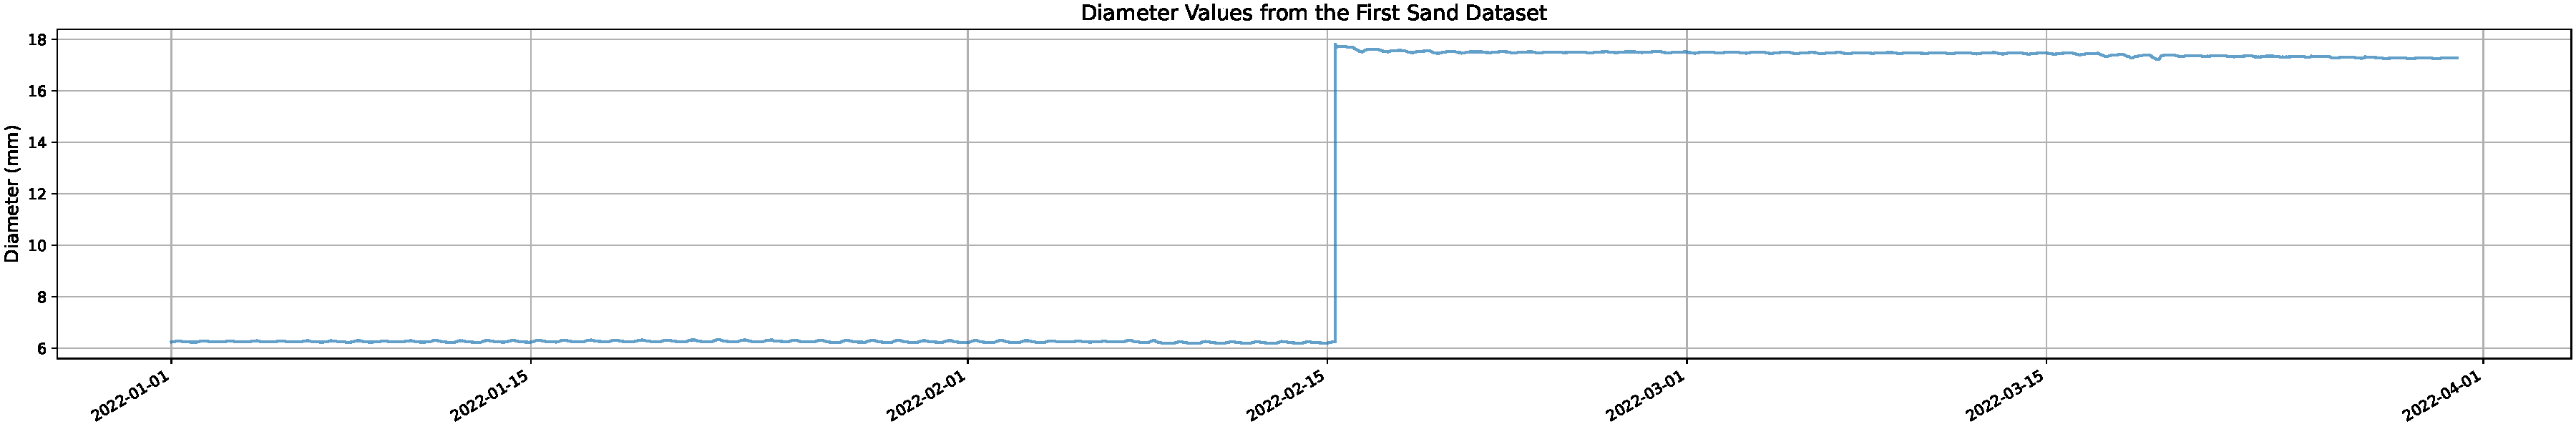
\includegraphics[width=15 cm]{5_ChapterDesign/figuras/1_DatasetIssues/Diameter_Sand_1}
    \caption{Example of Diameter Measurement Error in the First Sand Dataset}
    \label{Diameter_Sand_1}
\end{figure}

\begin{figure}[htbp]
    \centering
    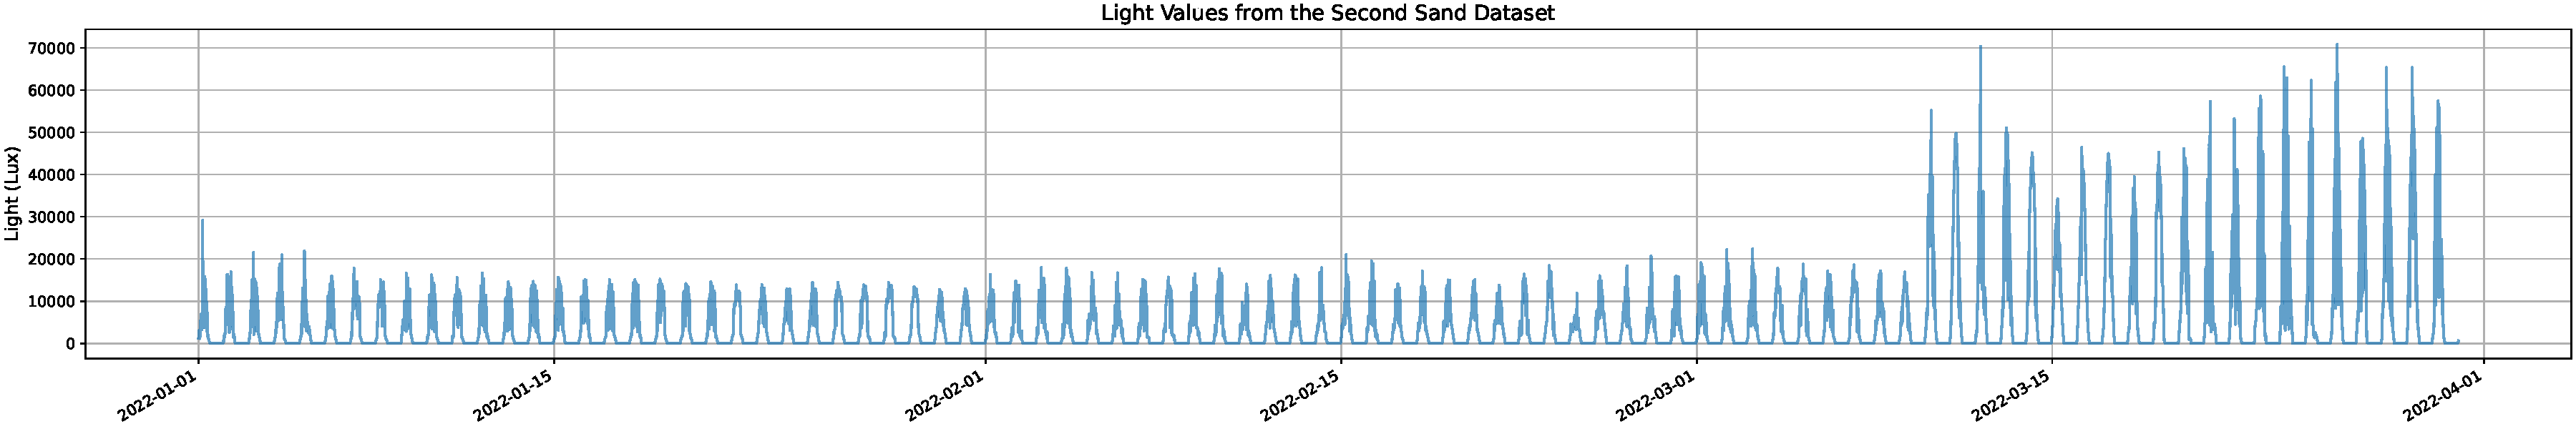
\includegraphics[width=15 cm]{5_ChapterDesign/figuras/1_DatasetIssues/Light_Sand_2}
    \caption{Example of Light Measurement Error in the Second Sand Dataset}
    \label{Light_Sand_2}
\end{figure}


\subsection{Structure}

The initial dataset provided by Ornavera was in the \texttt{.mat} format, which is commonly used for MATLAB. To facilitate data analysis and manipulation in Python, it was necessary to convert this data into a \texttt{.csv} file format. This conversion was advantageous because \texttt{.csv} files are universally supported and can be easily imported into Python libraries such as Pandas, making data manipulation and analysis straightforward. Additionally, CSV files are text-based, making them easy to inspect and modify with a simple text editor, and they offer efficiency benefits for large datasets due to their simple structure, which can be quickly parsed by Python libraries.

To perform the conversion, we wrote a MATLAB function named \texttt{mat\_to\_csv}, which loads the data from the \texttt{.mat} file, eliminates unnecessary fields, and writes the cleaned data to a \texttt{.csv} file. The function specifically targeted fields that were not relevant to our analysis, such as various identifiers and redundant measurements. Removing these fields helped streamline the dataset, ensuring that it was focused on the variables that were of interest for our study.

\begin{lstlisting}[language=Matlab,caption={MATLAB function to convert .mat file to .csv}, label=lst:mat_to_csv]
function mat_to_csv(mat_file, csv_file)
    % Load the data from the .mat file
    load(mat_file, 'val');
    
    % Eliminate the fields we are not interested in
    fields_to_eliminate = {'rid', 'cid','lid','vpd1','dd1','wtlux','alux','ecb1','ecp1','st2', 'p2', 'ec2', 'vwc2', 'ecb2', 'ecp2', 'st3', 'p3', 'ec3', 'vwc3', 'ecb3', 'ecp3','par','dli'};
    val_cleaned = val; % Create a copy of the original structure
    for i = 1:numel(fields_to_eliminate)
        val_cleaned = rmfield(val_cleaned, fields_to_eliminate{i});
    end
    
    % Convert the data from a structure to a table
    val_table = struct2table(val_cleaned);
    
    % Change the field names of the table
    new_names = {'Identificator', 'Date', 'Month','Day','Year','Hour','Minute','Second','Temperature','Relative_humidity', 'Light', 'Soil_temperature', 'Permittivity', 'Electroconductivity', 'Volumetric_water_content', 'Diameter', 'Battery_voltage'};
    val_table.Properties.VariableNames = new_names;
    
    % Write the data to a .csv file
    writetable(val_table, csv_file, 'Delimiter', ';');
end
\end{lstlisting}

The code effectively transformed the data from a complex structure into a more usable format by converting it into a table and renaming the fields to be more descriptive. The \texttt{.csv} file was then generated with a delimiter suitable for easy parsing in Python. This preparation step was crucial in setting the stage for efficient data handling and analysis in the subsequent phases of the project.

\subsection{Signal smoothing}

To achieve the signal smoothing, we use a Savitzky-Golay filter with a window size of 11 and a polynomial order of 2. The window size is set to 11, meaning that 11 adjacent data points are used to calculate each smoothed value. This implies that the filter takes these 11 points and fits a second-degree polynomial, also known as a parabola, to the data within each window, allowing the signal to be smoothed without losing its essential characteristics.

The \texttt{savgol\_filter} function generates a smoothed version of the input signal. By applying this filter, the smoothed signal exhibits a significant reduction in noise, making it more continuous and less fluctuating than the original signal. The smoothing process enhances the visualization and analysis of the underlying trends in the data, allowing important features to stand out more clearly. This can be clearly observed in the graphs presented in Figures \ref{Smoothing_Temperature}, \ref{Smoothing_Relative_humidity}, \ref{Smoothing_Light}, \ref{Smoothing_Soil_temperature}, \ref{Smoothing_Permittivity}, \ref{Smoothing_Electroconductivity}, and \ref{Smoothing_Diameter}.

\begin{figure}[htbp]
    \centering
    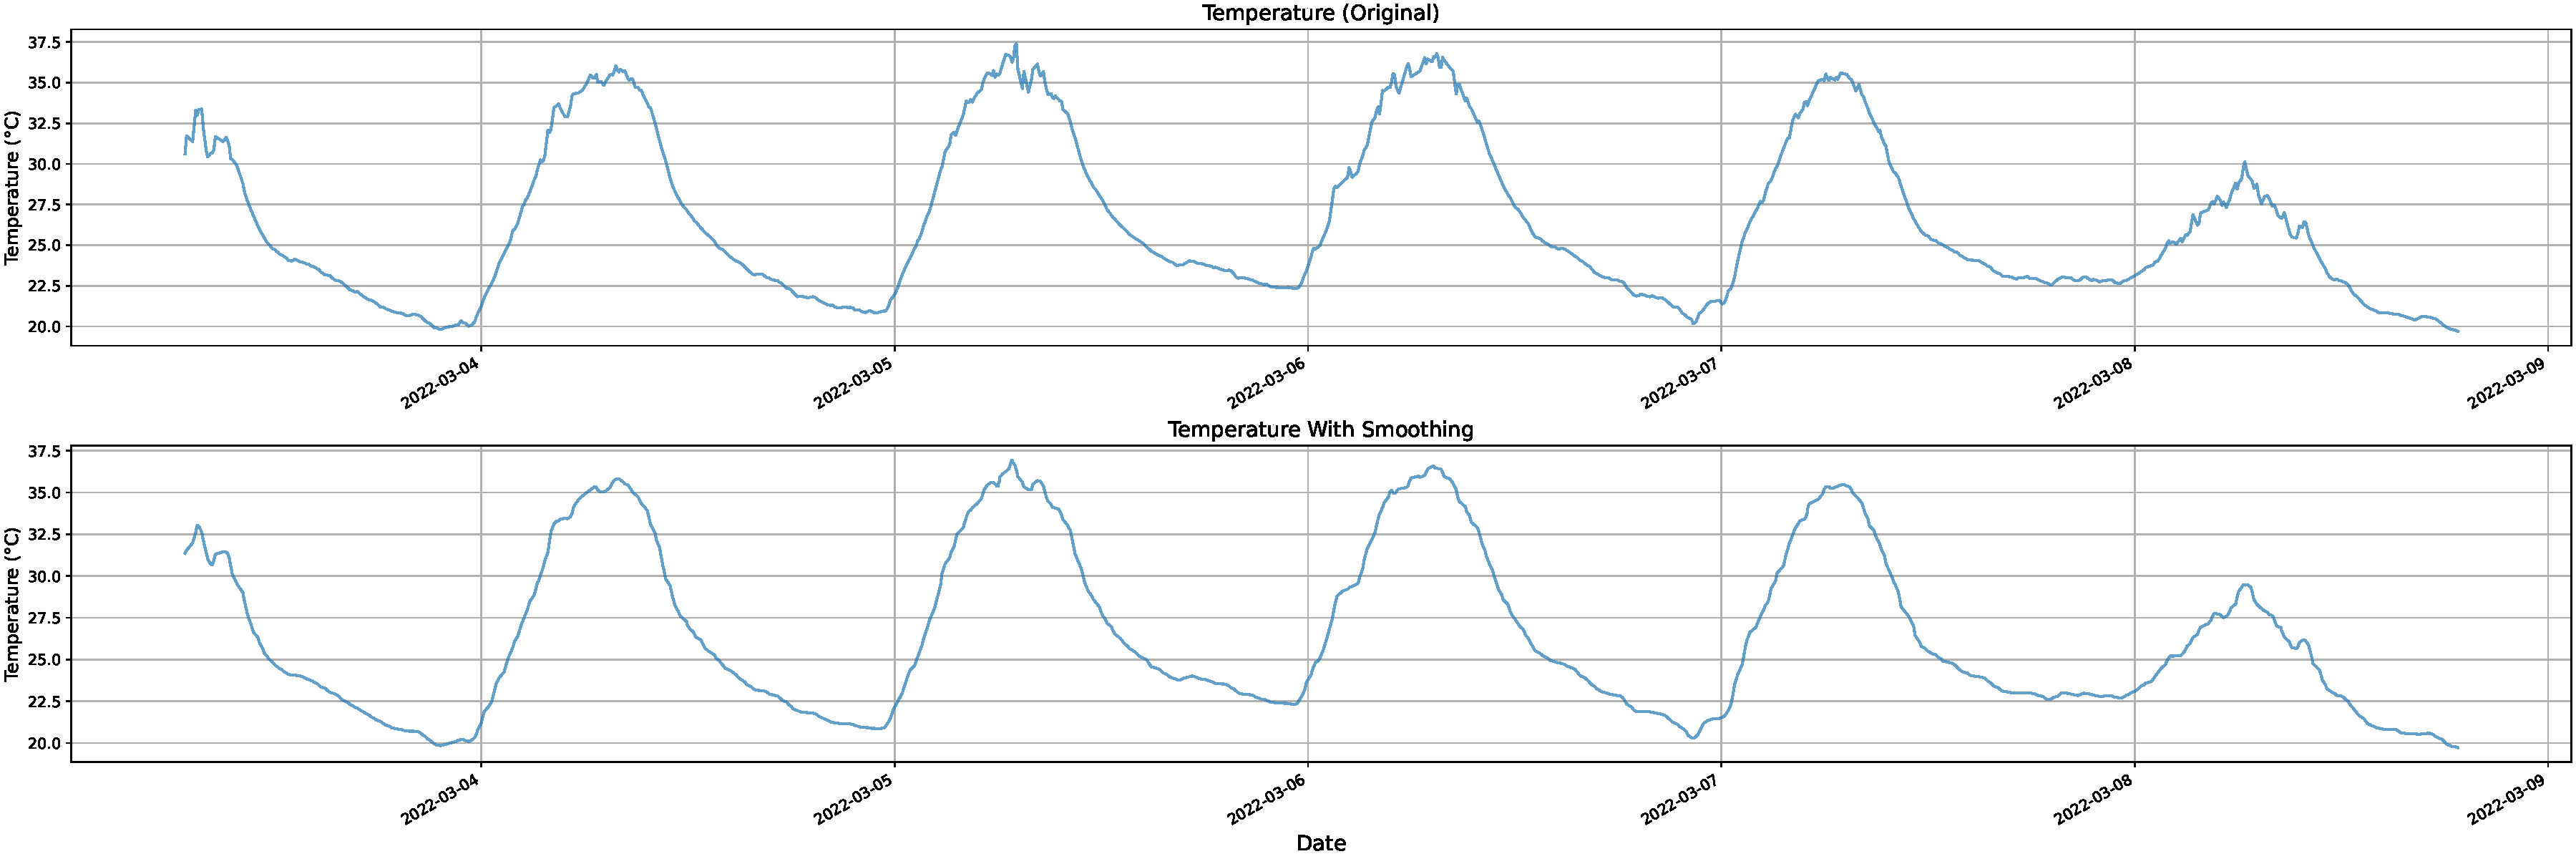
\includegraphics[width=15 cm]{5_ChapterDesign/figuras/2_Smoothing/Smoothing_Temperature}
    \caption{Original Temperature data (top) versus the Temperature smoothed data (bottom) after applying a Savitzky-Golay filter}
    \label{Smoothing_Temperature}
\end{figure}

\begin{figure}[htbp]
    \centering
    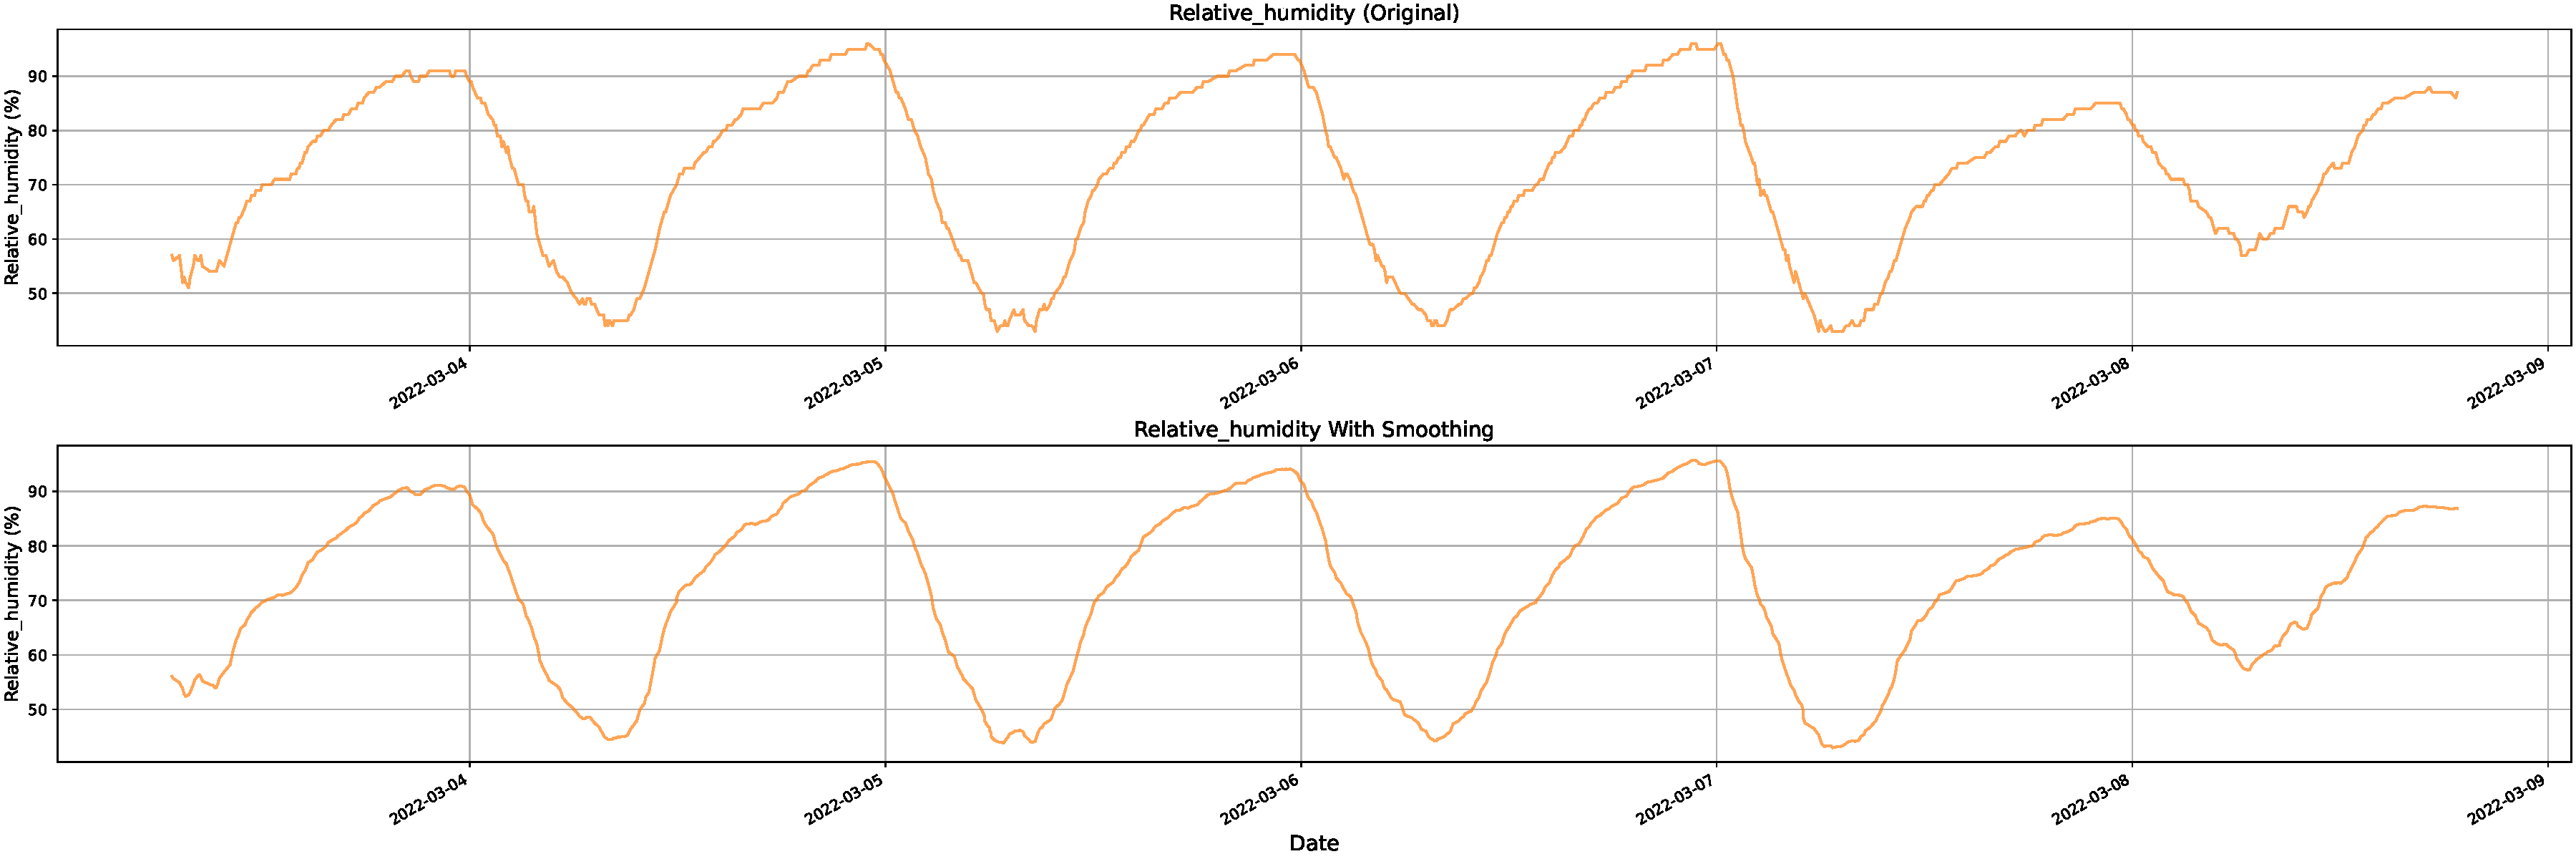
\includegraphics[width=15 cm]{5_ChapterDesign/figuras/2_Smoothing/Smoothing_Relative_humidity}
    \caption{Original Relative humidity data (top) versus the Relative humidity smoothed data (bottom) after applying a Savitzky-Golay filter}
    \label{Smoothing_Relative_humidity}
\end{figure}

\begin{figure}[htbp]
    \centering
    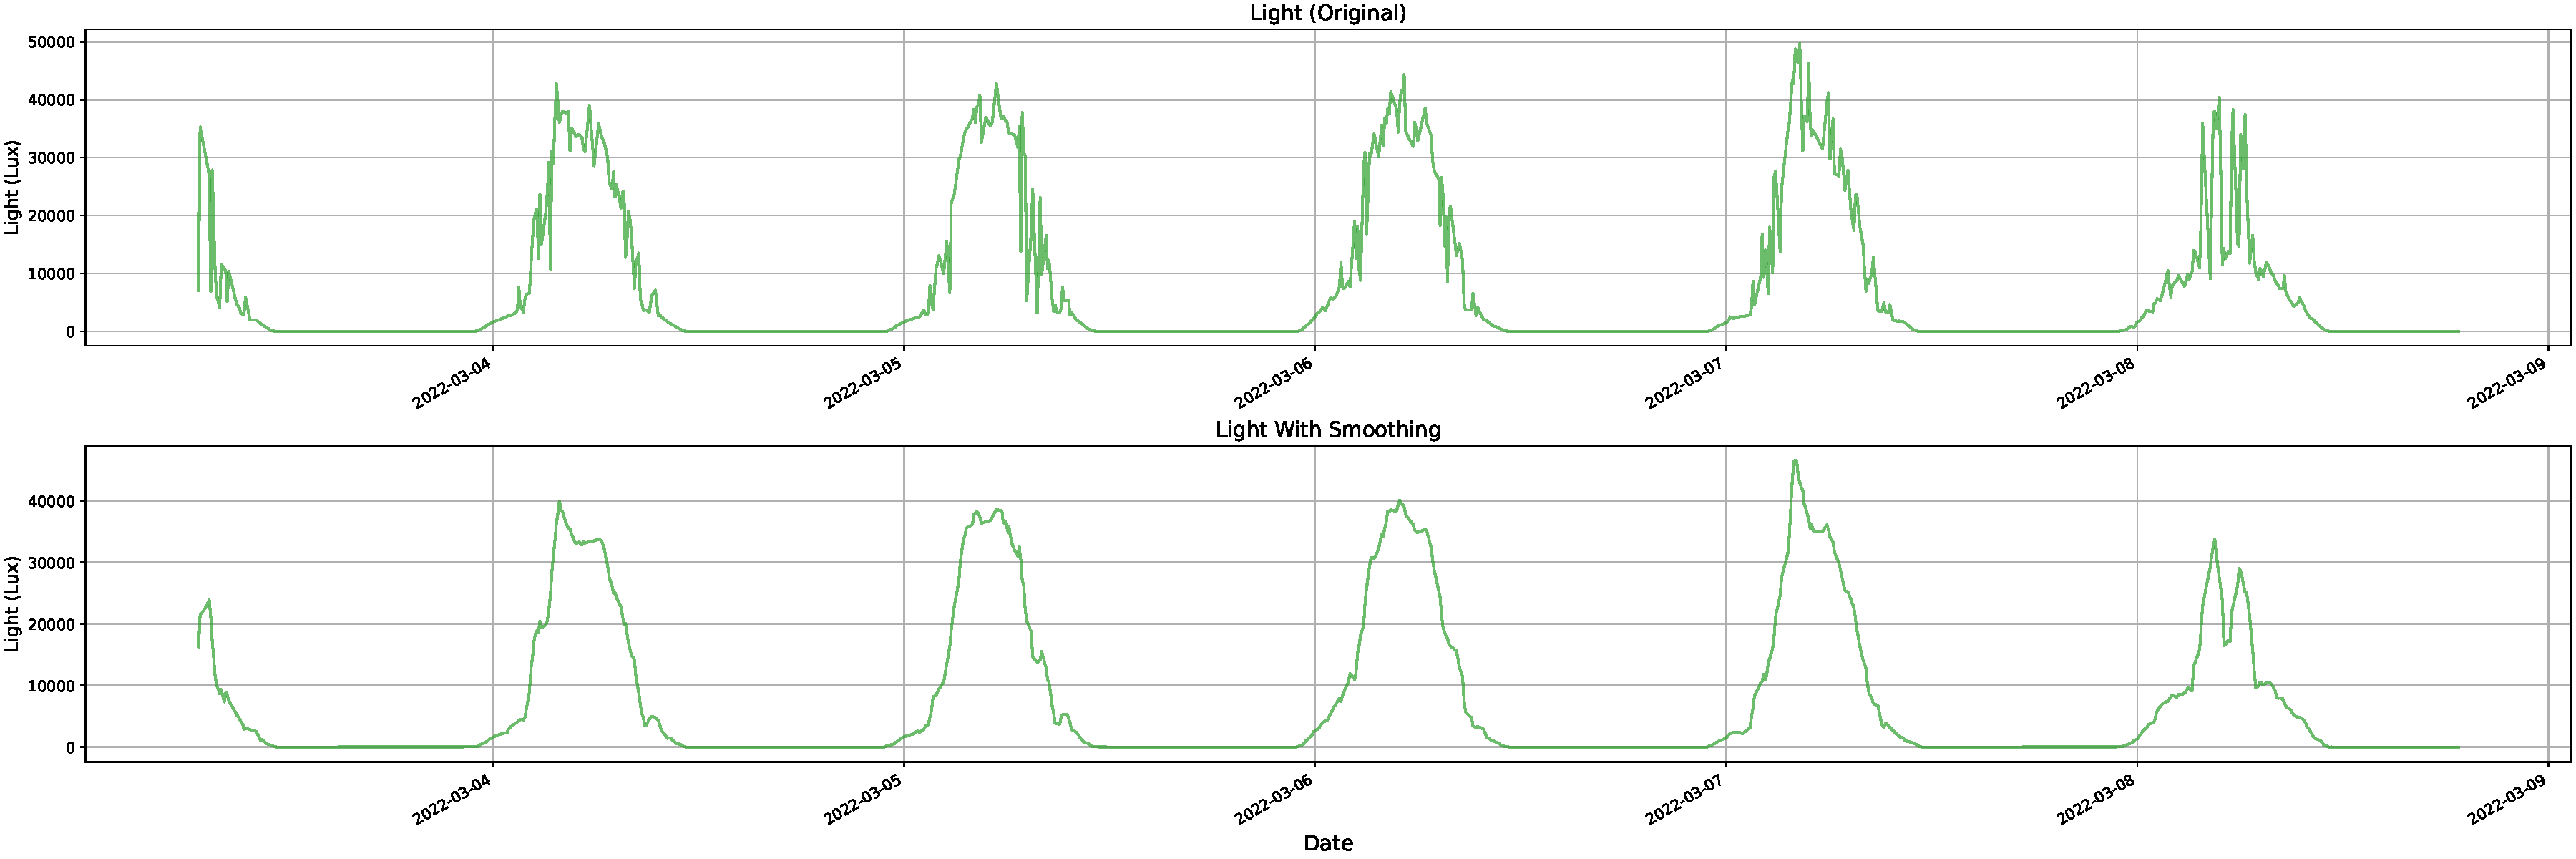
\includegraphics[width=15 cm]{5_ChapterDesign/figuras/2_Smoothing/Smoothing_Light}
    \caption{Original Light data (top) versus the Light smoothed data (bottom) after applying a Savitzky-Golay filter}
    \label{Smoothing_Light}
\end{figure}

\begin{figure}[htbp]
    \centering
    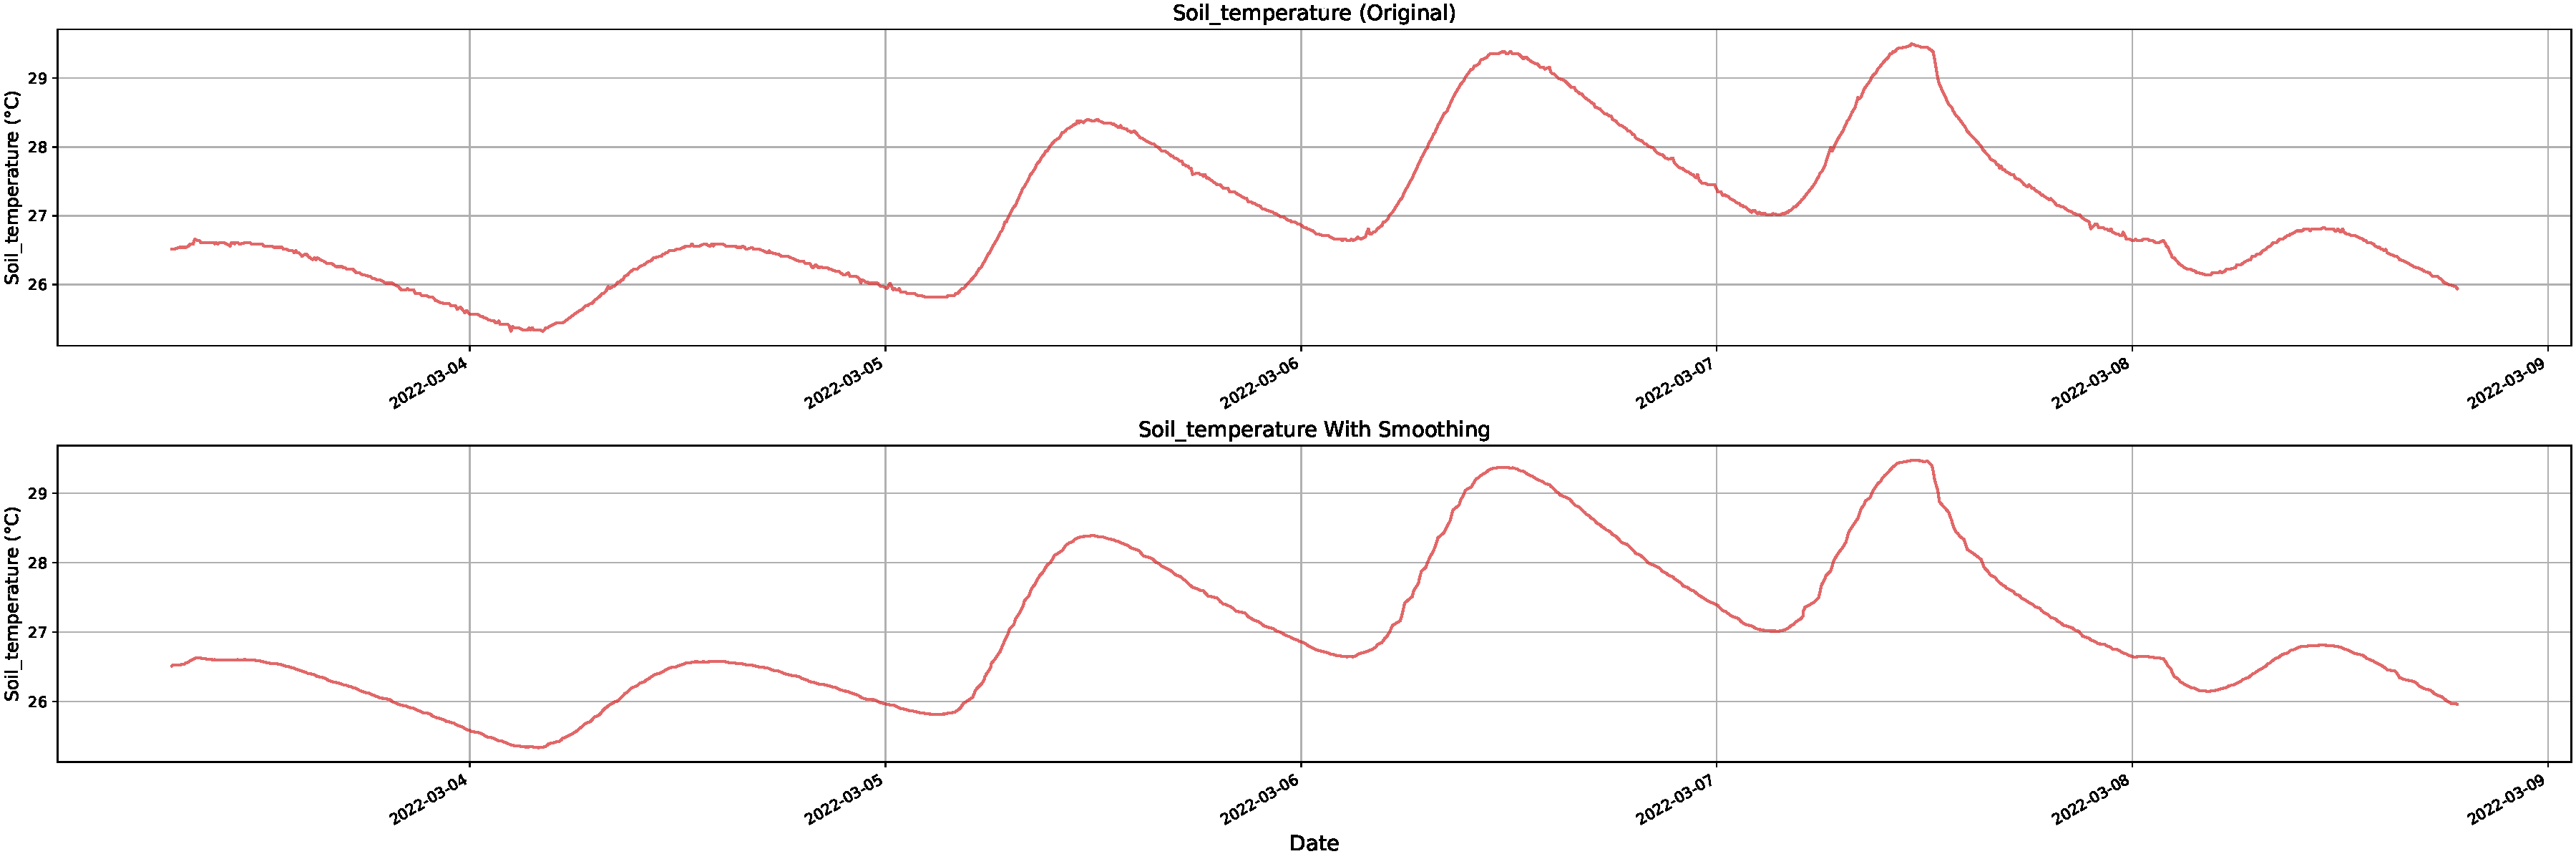
\includegraphics[width=15 cm]{5_ChapterDesign/figuras/2_Smoothing/Smoothing_Soil_temperature}
    \caption{Original Soil temperature data (top) versus the Soil temperature smoothed data (bottom) after applying a Savitzky-Golay filter}
    \label{Smoothing_Soil_temperature}
\end{figure}

\begin{figure}[htbp]
    \centering
    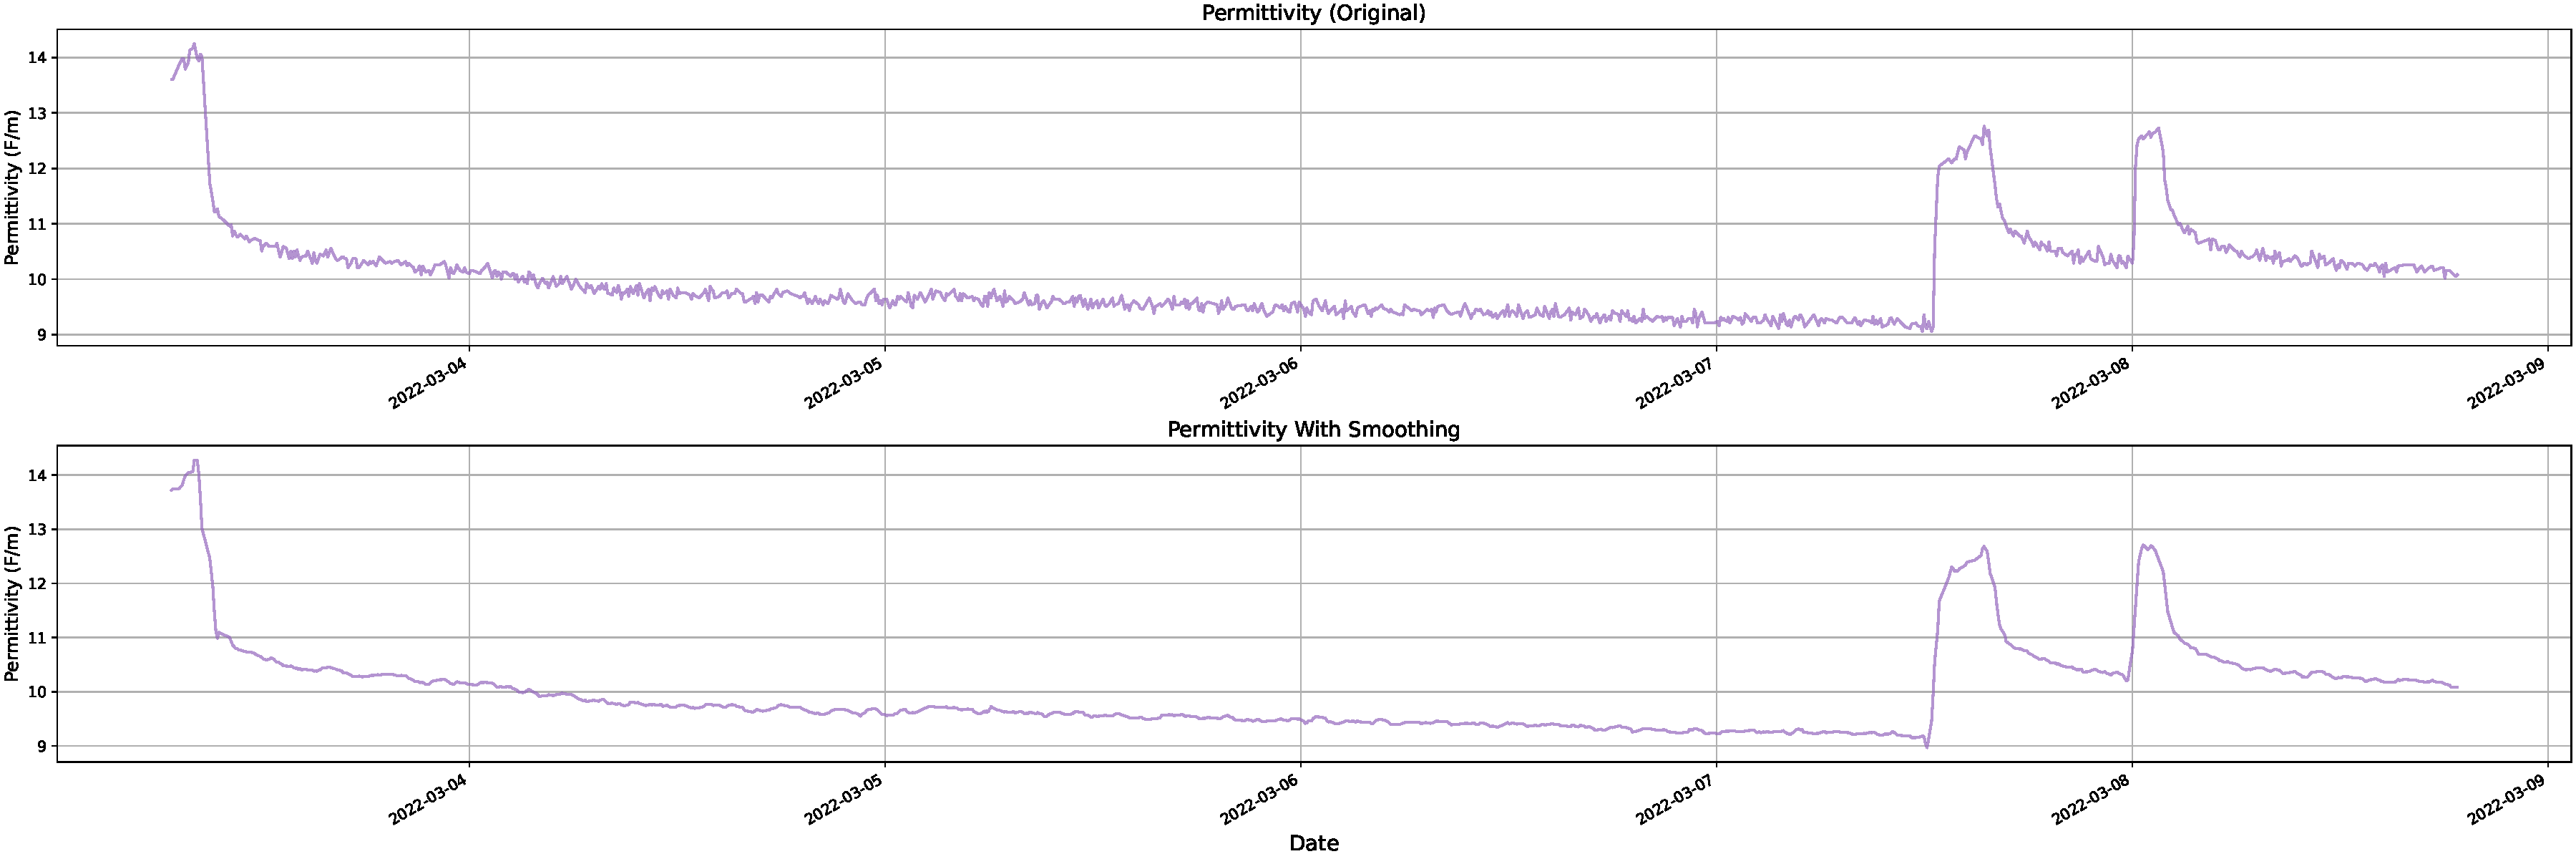
\includegraphics[width=15 cm]{5_ChapterDesign/figuras/2_Smoothing/Smoothing_Permittivity}
    \caption{Original Permittivity data (top) versus the Permittivity smoothed data (bottom) after applying a Savitzky-Golay filter}
    \label{Smoothing_Permittivity}
\end{figure}

\begin{figure}[htbp]
    \centering
    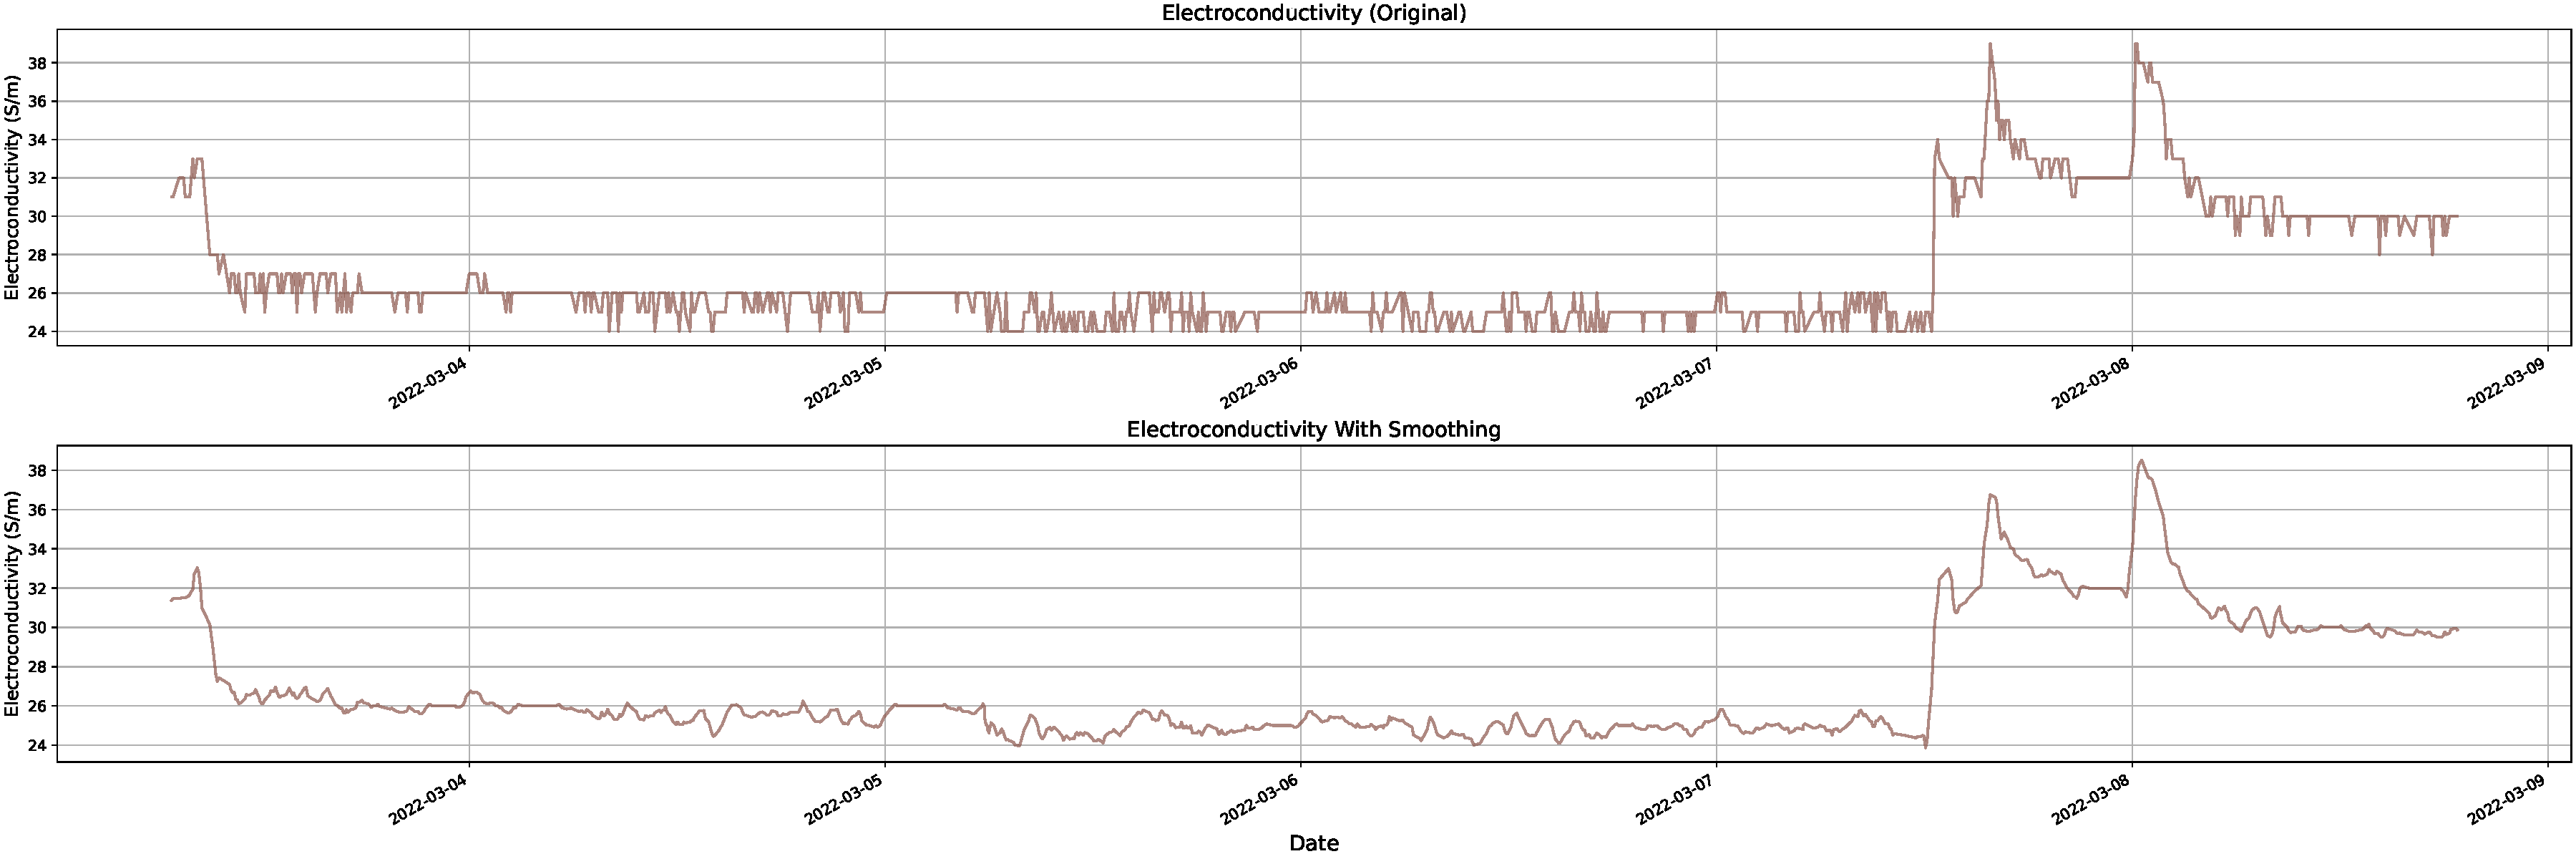
\includegraphics[width=15 cm]{5_ChapterDesign/figuras/2_Smoothing/Smoothing_Electroconductivity}
    \caption{Original Electroconductivity data (top) versus the Electroconductivity smoothed data (bottom) after applying a Savitzky-Golay filter}
    \label{Smoothing_Electroconductivity}
\end{figure}

\begin{figure}[htbp]
    \centering
    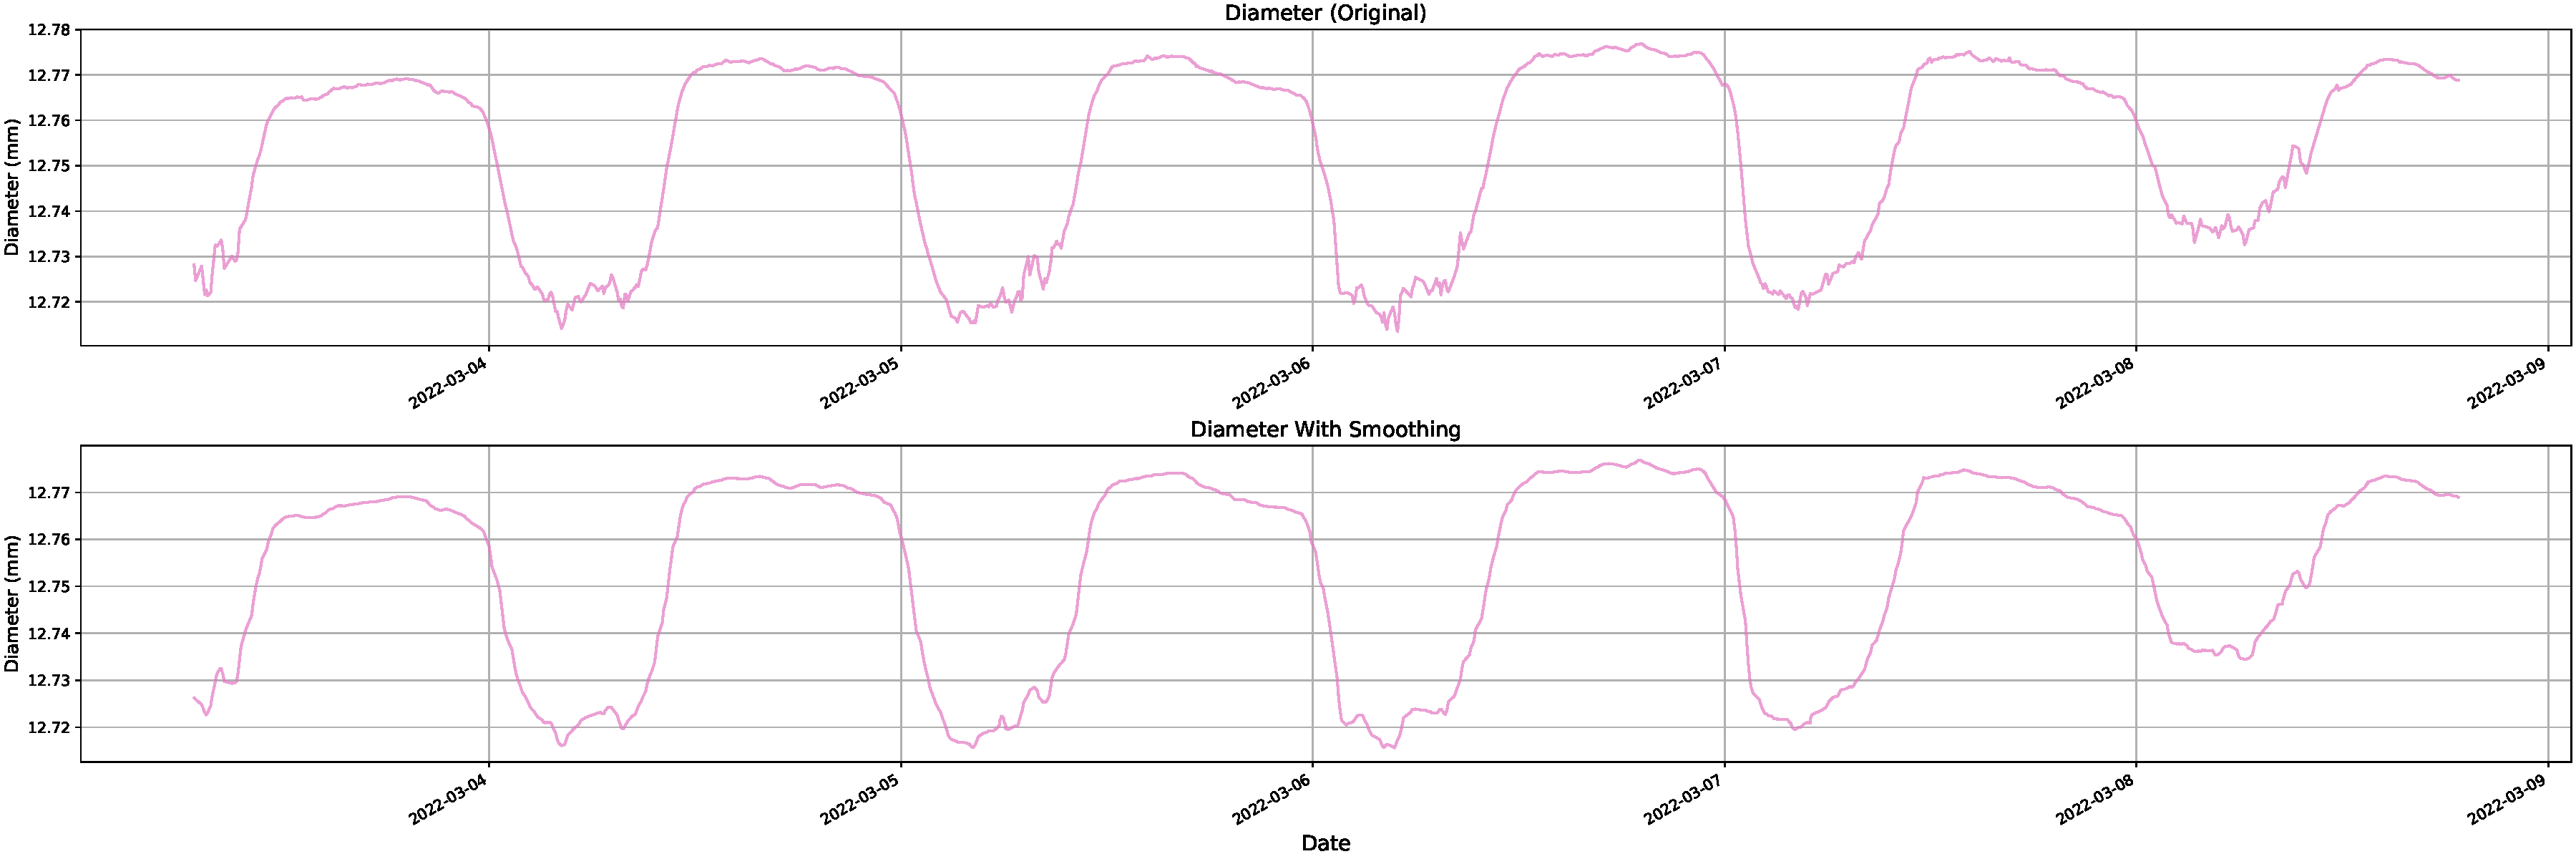
\includegraphics[width=15 cm]{5_ChapterDesign/figuras/2_Smoothing/Smoothing_Diameter}
    \caption{Original Diameter data (top) versus the Diameter smoothed data (bottom) after applying a Savitzky-Golay filter}
    \label{Smoothing_Diameter}
\end{figure}

\subsection{Elimination of the Trend}

In time series analysis, the elimination of the trend is a preprocessing technique used to make the series more stationary by removing long-term trends that could bias the analysis. The trend in a time series represents a systematic direction that can interfere with detecting relevant patterns, such as cycles or seasonalities. However, trend elimination is not always necessary or convenient, as some series require retaining their trend to obtain accurate and useful results in the analysis.

Eliminating the trend offers several advantages. First, it improves the stationarity of the series, which is crucial for applying many forecasting methods. Stationary series allow for the application of statistical models with greater ease and precision. Second, removing the trend reduces unnecessary variability, as the trend can introduce changes not related to the internal dynamics of the system under analysis. By removing it, intrinsic patterns become more apparent. Additionally, in some cases, analyzing variations around a fixed trend can offer a clearer interpretation of the data. For example, it may be more useful to observe fluctuations around a constant average than to analyze changes in the context of continuous growth.

On the other hand, the trend should be retained when it has significant interpretative value or is important for future prediction. In series where the trend is part of relevant seasonal or cyclical behavior for the analysis, it is crucial to maintain it. Also, in variables representing natural growth, such as population growth, the trend provides valuable information that should be preserved.

In this project, we evaluated each variable individually to decide if trend elimination was appropriate.

For the variable \textbf{Temperature}, we chose to retain the trend. Temperature often shows seasonal trends that are relevant for analysis. The trend in this variable may reflect natural and seasonal climate changes, so removing it could lead to the loss of crucial information about these patterns.

For the variable \textbf{Relative Humidity}, we chose to retain the trend. Relative humidity presents significant seasonal variations that may be affected by climate changes, and the trend in this variable provides valuable information on how environmental conditions evolve over time.

For the variable \textbf{Light}, we chose to retain the trend. Ambient light is a factor that can show significant diurnal and seasonal trends, and analyzing these trends is vital for understanding how light availability affects plant growth and overall health.

For the variable \textbf{Soil Temperature}, we chose to retain the trend. This variable follows patterns similar to air temperature, with important seasonal variations for plant health. The trend may indicate seasonal changes influencing soil biological activity.

For the variable \textbf{Permittivity}, we chose to retain the trend. Soil permittivity reflects the soil's ability to store moisture, and its change over time can indicate changes in soil conditions. Retaining the trend helps us observe these natural variations, which are crucial for soil condition analysis.

For the variable \textbf{Electroconductivity}, we chose to retain the trend. We did not remove the trend because soil electrical conductivity is related to the amount of dissolved salts in the soil and can change with the application of fertilizers or irrigation. The trend in this variable can provide information on the evolution of soil salinity, which is vital for agricultural management.

However, for the variable \textbf{Diameter}, we decided to remove the trend. Our main interest was in analyzing diameter variations to detect signs of disease or stress in the plant rather than its constant growth. By removing the trend, we could focus on fluctuations in diameter around its general trend, identifying possible anomalies that might indicate plant health issues.

To remove the trend in the \textbf{Diameter} variable, we applied a smoothing method using a moving average. This approach involves calculating the average of the data within a fixed-size window and subtracting that average from the original values. The mathematical formula describing this process is:

\begin{equation}
D_t^{\text{adjusted}} = D_t - \frac{1}{n} \sum_{i=t-n+1}^{t} D_i \text{ ,}
\end{equation}

where:
\begin{itemize}
    \item $D_t^{\text{adjusted}}$ is the adjusted diameter value at time $t$.
    \item $D_t$ is the original diameter value at time $t$.
    \item $n$ is the window size (100 in this case).
    \item $\sum$ represents the sum of the values within the moving window.
\end{itemize}

In our case, we used a window of 100 data points. Below is a comparison of the diameter before and after removing the trend (see Figure \ref{WithoutTrend_Diameter}).

\begin{figure}[htbp]
    \centering
    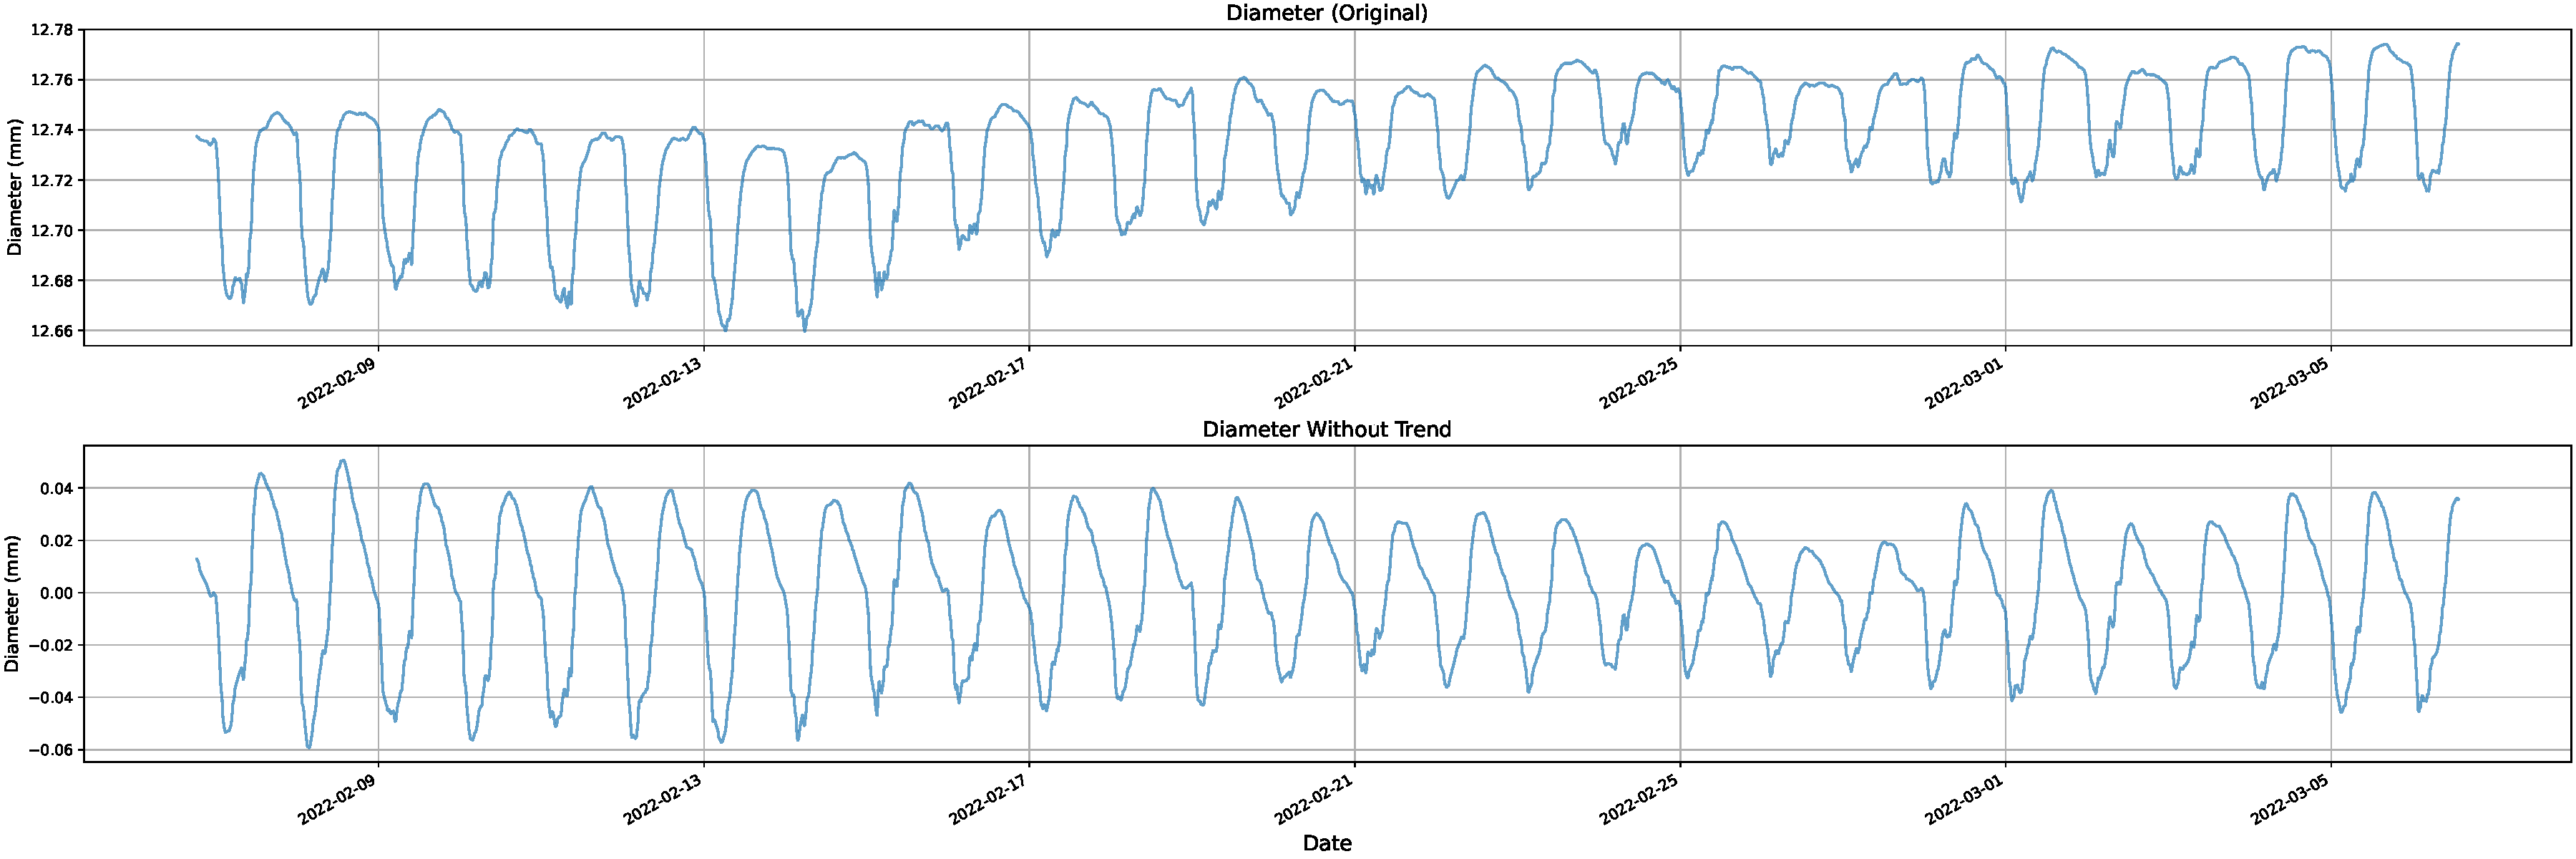
\includegraphics[width=15 cm]{5_ChapterDesign/figuras/3_Trend/WithoutTrend_Diameter}
    \caption{Original Diameter data (top) versus the Diameter without trend (bottom)}
    \label{WithoutTrend_Diameter}
\end{figure}


\subsection{Elimination of NaN Values}

The elimination of NaN values is a crucial step in data preprocessing for time series. In our case, two main reasons for the presence of NaN values in the dataset were identified.

First, when applying a moving window of 100 data points to remove trends, the first 100 data points of the series resulted in NaN values. This occurred because, when calculating the moving average, there were not enough preceding data points to determine a value for the initial points in the series, leading to NaN values at those positions.

The second reason for NaN values was the presence of errors in the measurement sensors. During data collection, failures or disconnections in the sensors caused incomplete records, resulting in NaN values in the original dataset. Below is an image indicating the location of the 51 specific measurements where NaN values were detected due to sensor errors (see Figure \ref{nan_index_distribution}).

\begin{figure}[htbp]
    \centering
    
\includegraphics[width=15 cm]{5_ChapterDesign/figuras/4_IndexNan/nan_index_distribution.pdf}
    \caption{Measurements with NaN values distribution}
    \label{nan_index_distribution}
\end{figure}


Eliminating these NaN values was essential to ensure the quality and accuracy of the subsequent analysis, preventing incomplete or incorrect data from affecting the results of our study.


\subsection{Normalization of data}

To prepare the data, we applied a normalization process using the MinMaxScaler class from the sklearn library. Normalization is a crucial technique in data analysis that transforms variables to share a common scale. This adjustment is essential to minimize the impact of differences in the magnitude of variables on the analysis, allowing for a more equitable comparison between them.

The MinMaxScaler class performs Min-Max normalization, which adjusts the data to a specific range, typically between 0 and 1. In our case, we used this class to rescale all the variables in the data matrix to this 0 to 1 range.

Normalizing input data is vital for improving the accuracy and performance of machine learning models. Without proper normalization, variables with extremely high or low values can dominate the training process, potentially resulting in a less effective model. Additionally, normalizing the data can accelerate the convergence of the neural network during training, reducing the time needed for this process.

\subsection{Transforming Irregular Time Series to Regular Time Series}

Another significant challenge was that the measurements in the dataset were taken at irregular time intervals, resulting in an "irregular time series". In such a series, data points do not occur at consistent, predictable intervals, complicating analysis and model training. The time intervals between measurements varied, which is common in real-world data collection due to various operational constraints. Some periods had dense data collection, while others were sparse, affecting the analysis and modeling of temporal patterns.

To address this challenge, it was essential to transform the irregular time series into a regular one, compatible with the Hugging Face Transformers library. This library requires time series data to be defined with a start date and uniform time intervals. To achieve this, we employed a process known as time resampling.

We started by determining a suitable resampling frequency based on the average interval between consecutive measurements. With this frequency set, we used the resample method to aggregate data points into the new regular intervals by calculating the mean within each interval. This process smoothed out variations and preserved the central tendency of the data, resulting in a more consistent time series.

After resampling, we addressed the issue of missing values that often arise during this process. To maintain continuity in the dataset, we applied interpolation, which estimates intermediate values between data points. This step ensured that the time series was continuous and free of gaps, preserving the temporal structure and making the dataset ready for further analysis.

While this approach introduces a degree of approximation, the disadvantages are minimal, and the method provides a reasonably accurate representation of the underlying data. The resulting uniform time series simplified the dataset, making it easier to handle with various analytical tools and libraries while enabling accurate model training and forecasting.

Figures \ref{comparison_Temperature}, \ref{comparison_Relative_humidity}, \ref{comparison_Light}, \ref{comparison_Soil_temperature}, \ref{comparison_Permittivity}, \ref{comparison_Electroconductivity}, and \ref{comparison_Diameter} present comparisons of the measurements with both the original irregular time series and the resampled uniform time series.


\begin{figure}[htbp]
    \centering
    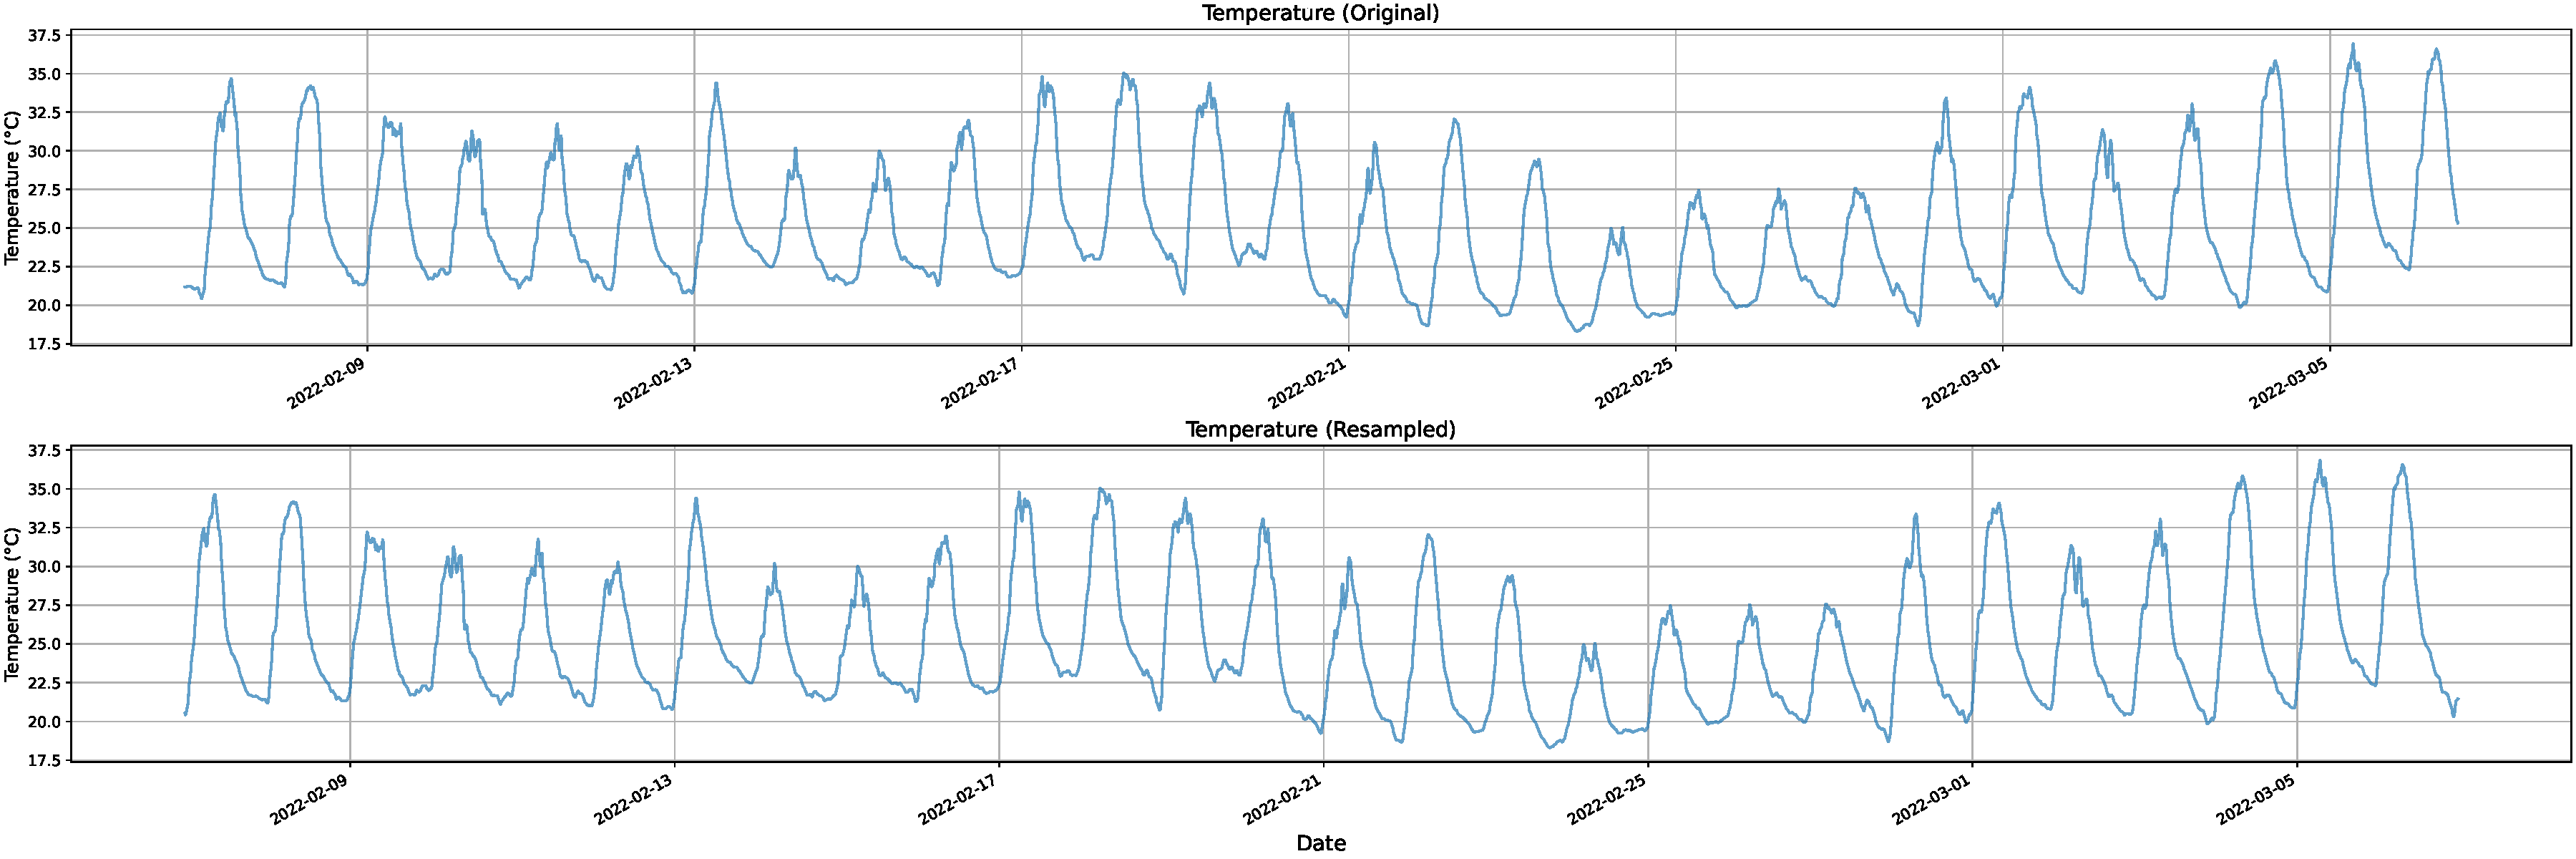
\includegraphics[width=15 cm]{5_ChapterDesign/figuras/5_Irregular/comparison_Temperature.pdf}
    \caption{Comparison of the original Temperature irregular time series and the resampled Temperature uniform time series}
    \label{comparison_Temperature}
\end{figure}

\begin{figure}[htbp]
    \centering
    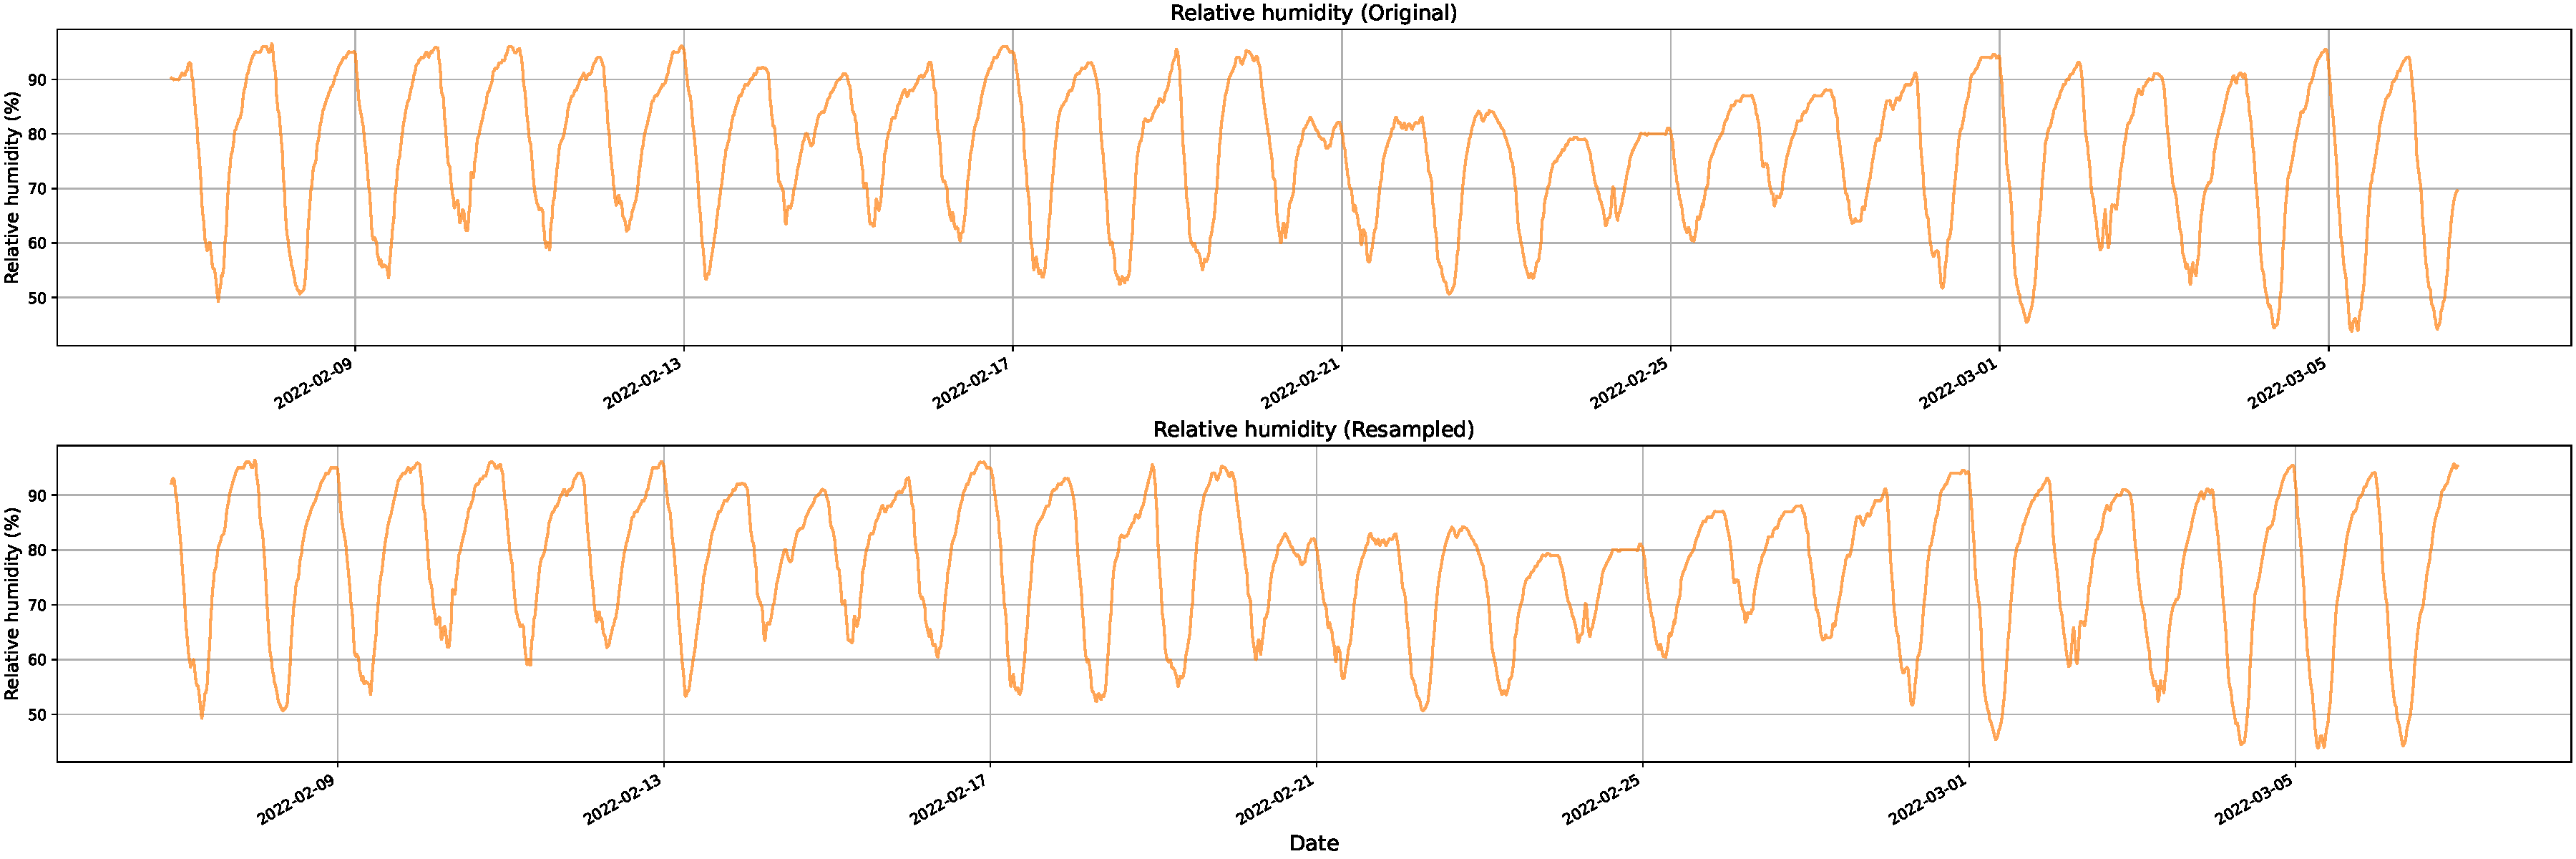
\includegraphics[width=15 cm]{5_ChapterDesign/figuras/5_Irregular/comparison_Relative_humidity.pdf}
    \caption{Comparison of the original Relative Humidity irregular time series and the resampled Relative Humidity uniform time series}
    \label{comparison_Relative_humidity}
\end{figure}

\begin{figure}[htbp]
    \centering
    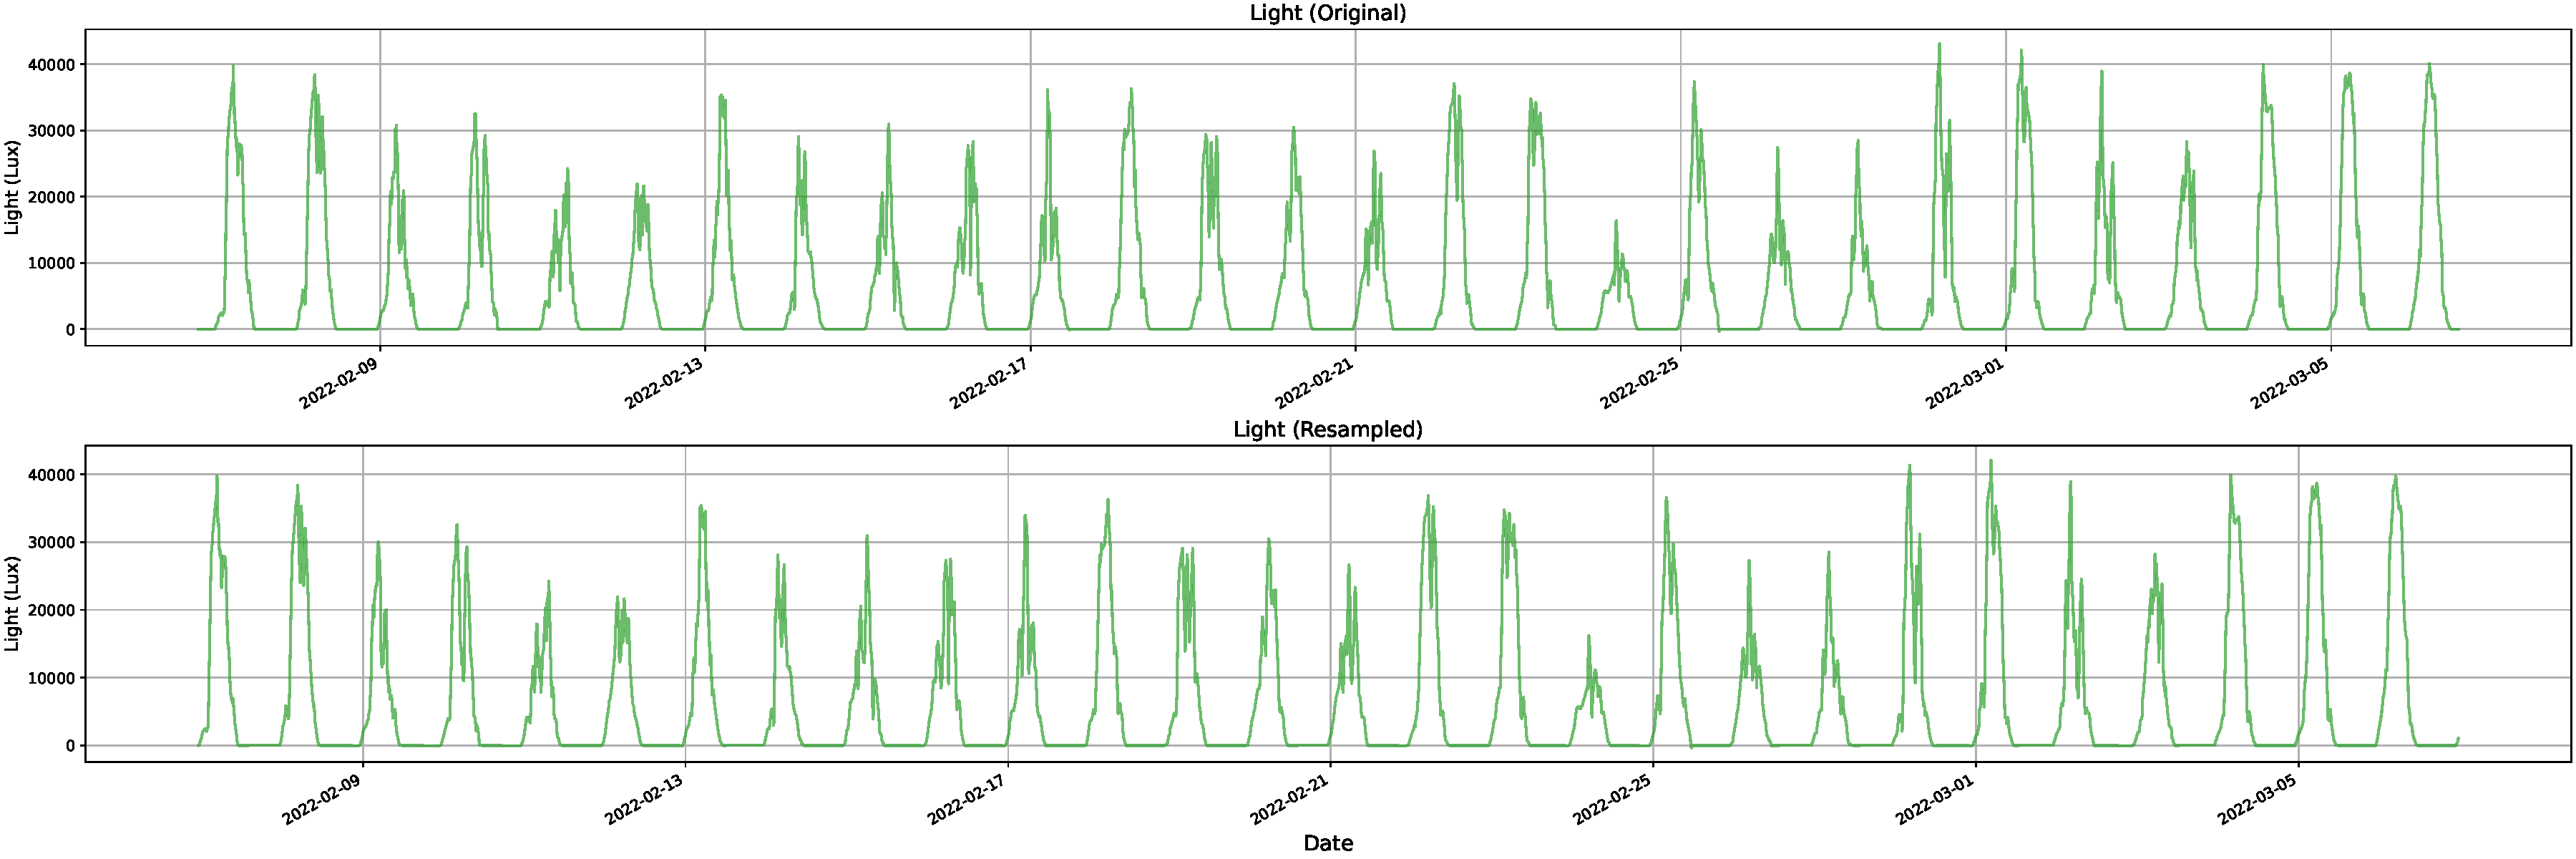
\includegraphics[width=15 cm]{5_ChapterDesign/figuras/5_Irregular/comparison_Light.pdf}
    \caption{Comparison of the original Light irregular time series and the resampled Light uniform time series}
    \label{comparison_Light}
\end{figure}

\begin{figure}[htbp]
    \centering
    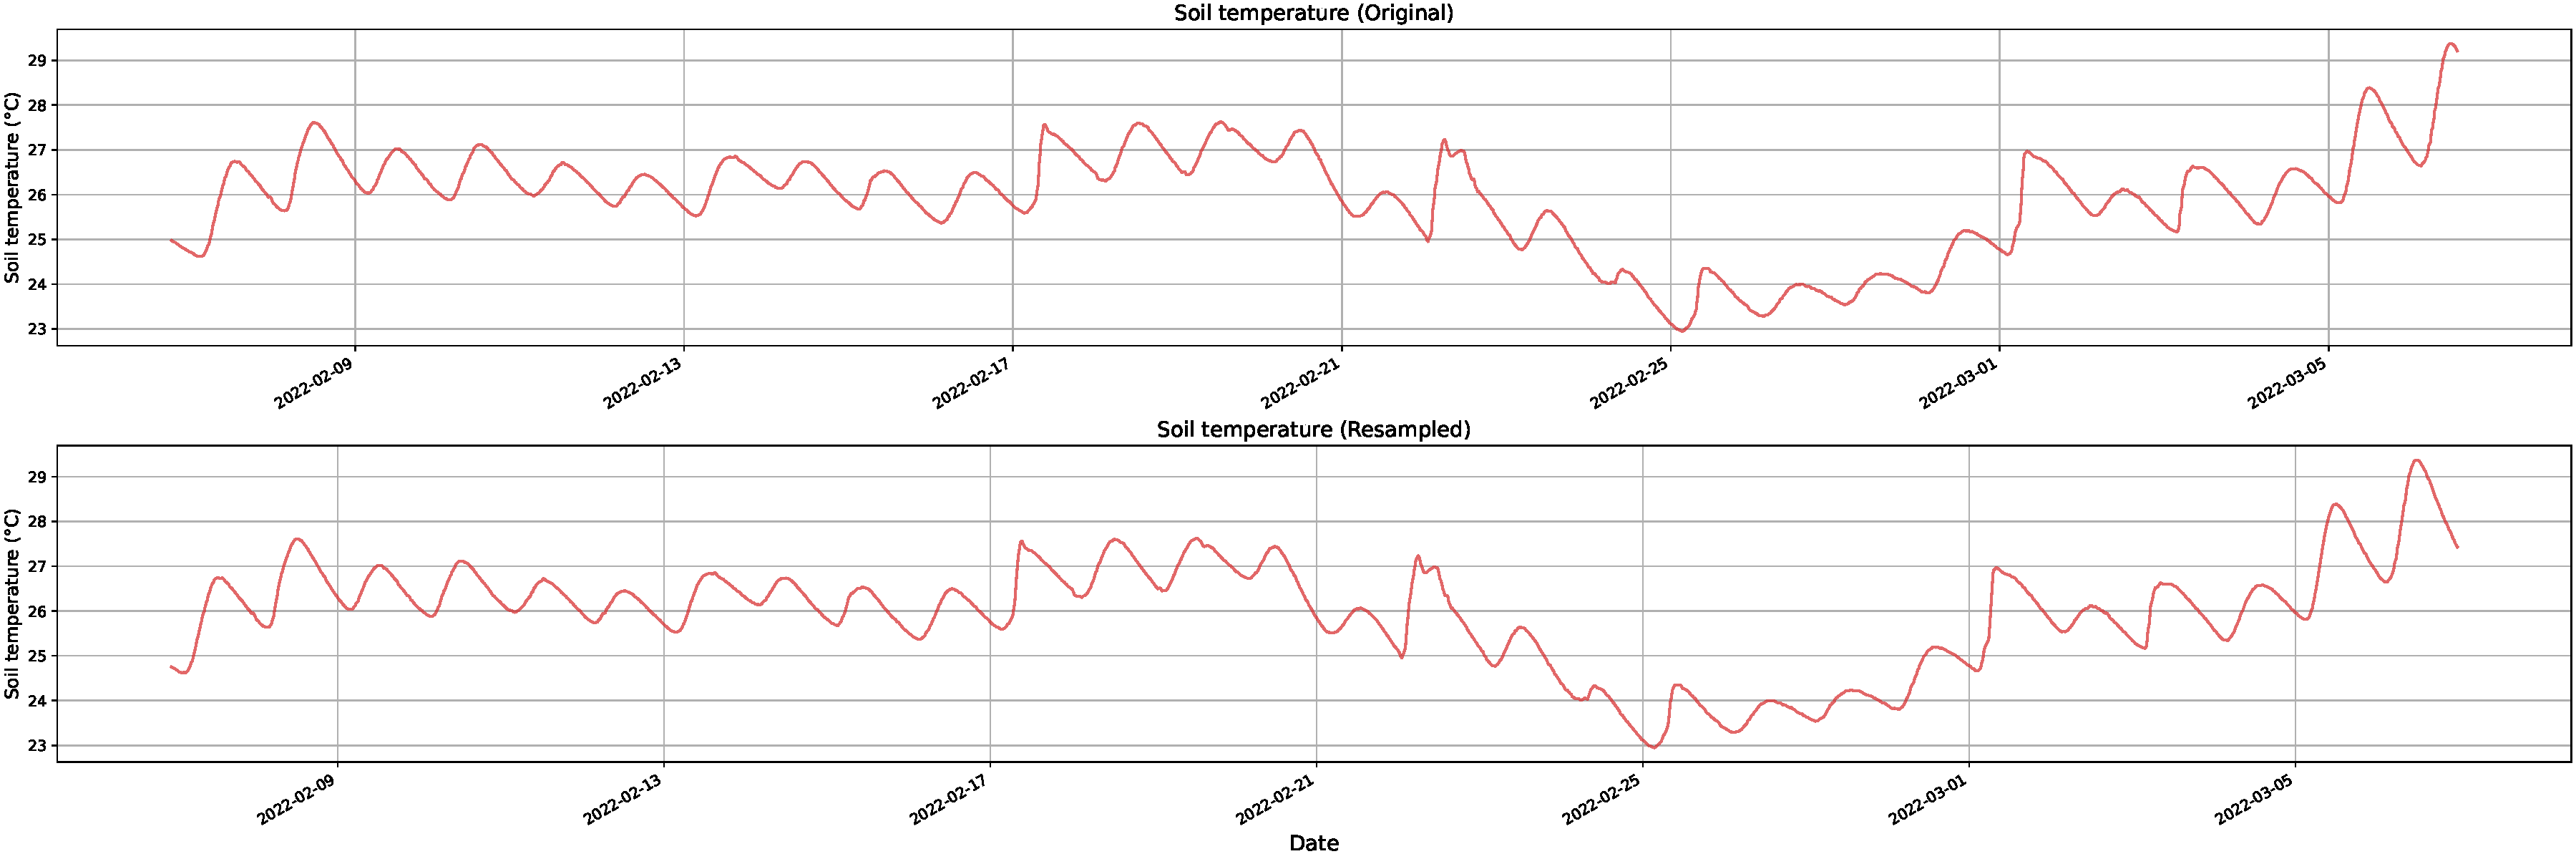
\includegraphics[width=15 cm]{5_ChapterDesign/figuras/5_Irregular/comparison_Soil_temperature.pdf}
    \caption{Comparison of the original Soil Temperature irregular time series and the resampled Soil Temperature uniform time series}
    \label{comparison_Soil_temperature}
\end{figure}

\begin{figure}[htbp]
    \centering
    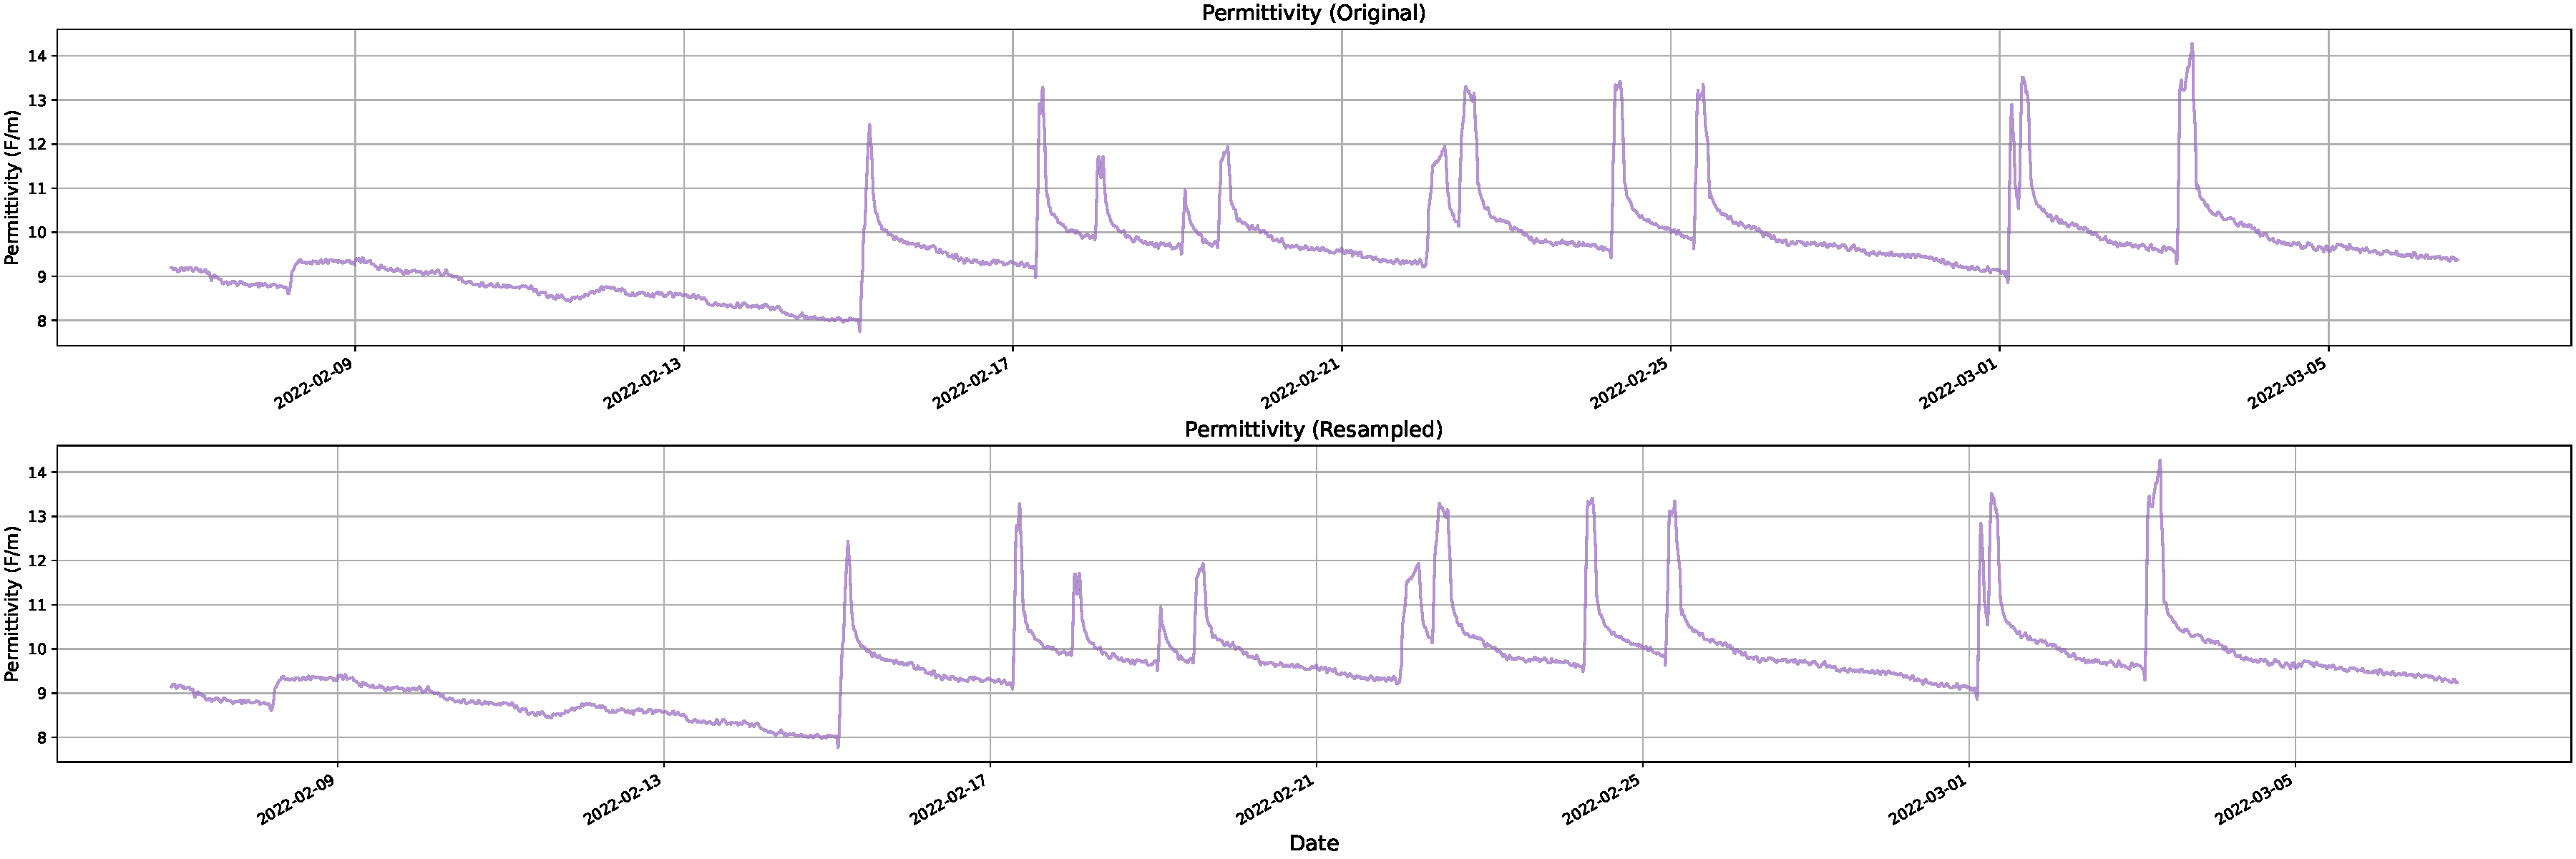
\includegraphics[width=15 cm]{5_ChapterDesign/figuras/5_Irregular/comparison_Permittivity.pdf}
    \caption{Comparison of the original Permittivity irregular time series and the resampled Permittivity uniform time series}
    \label{comparison_Permittivity}
\end{figure}

\begin{figure}[htbp]
    \centering
    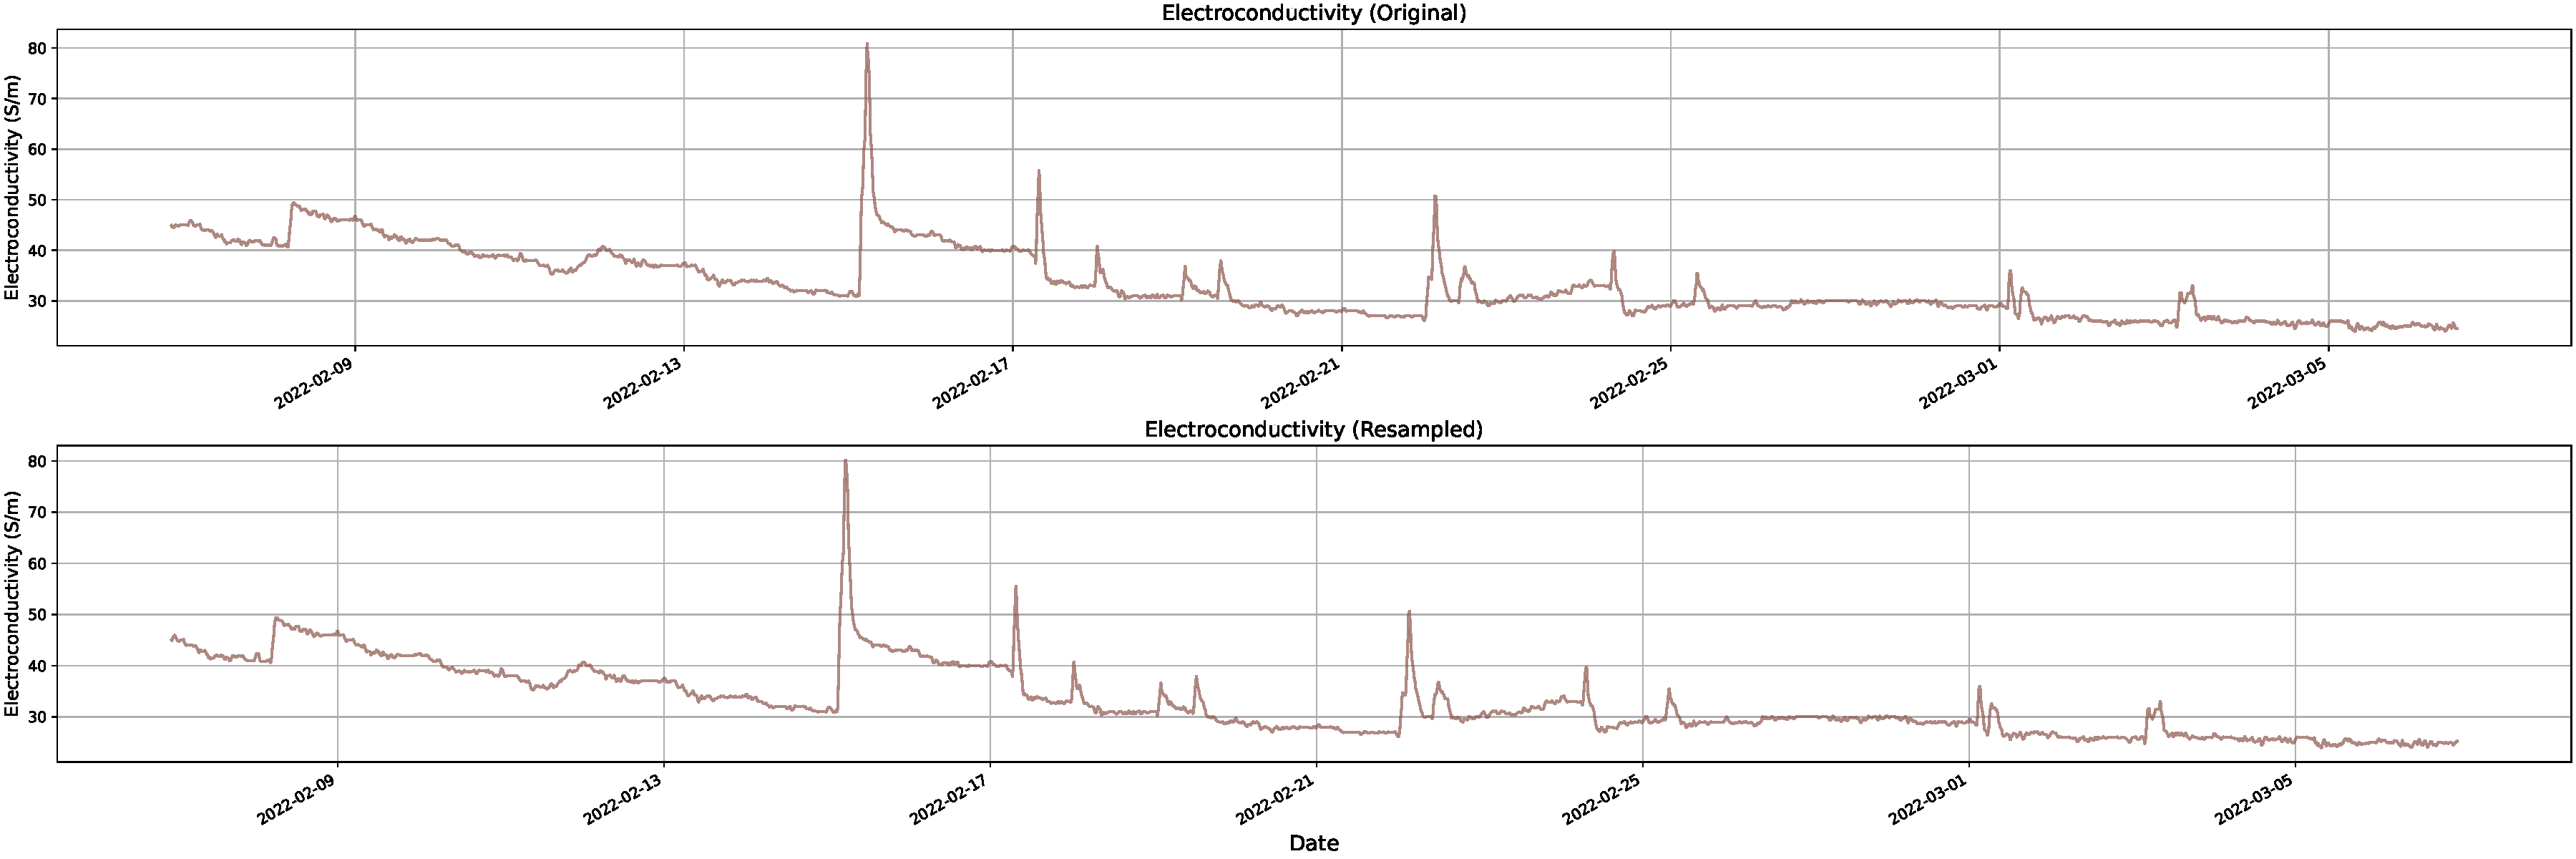
\includegraphics[width=15 cm]{5_ChapterDesign/figuras/5_Irregular/comparison_Electroconductivity.pdf}
    \caption{Comparison of the original Electroconductivity irregular time series and the resampled Electroconductivity uniform time series}
    \label{comparison_Electroconductivity}
\end{figure}

\begin{figure}[htbp]
    \centering
    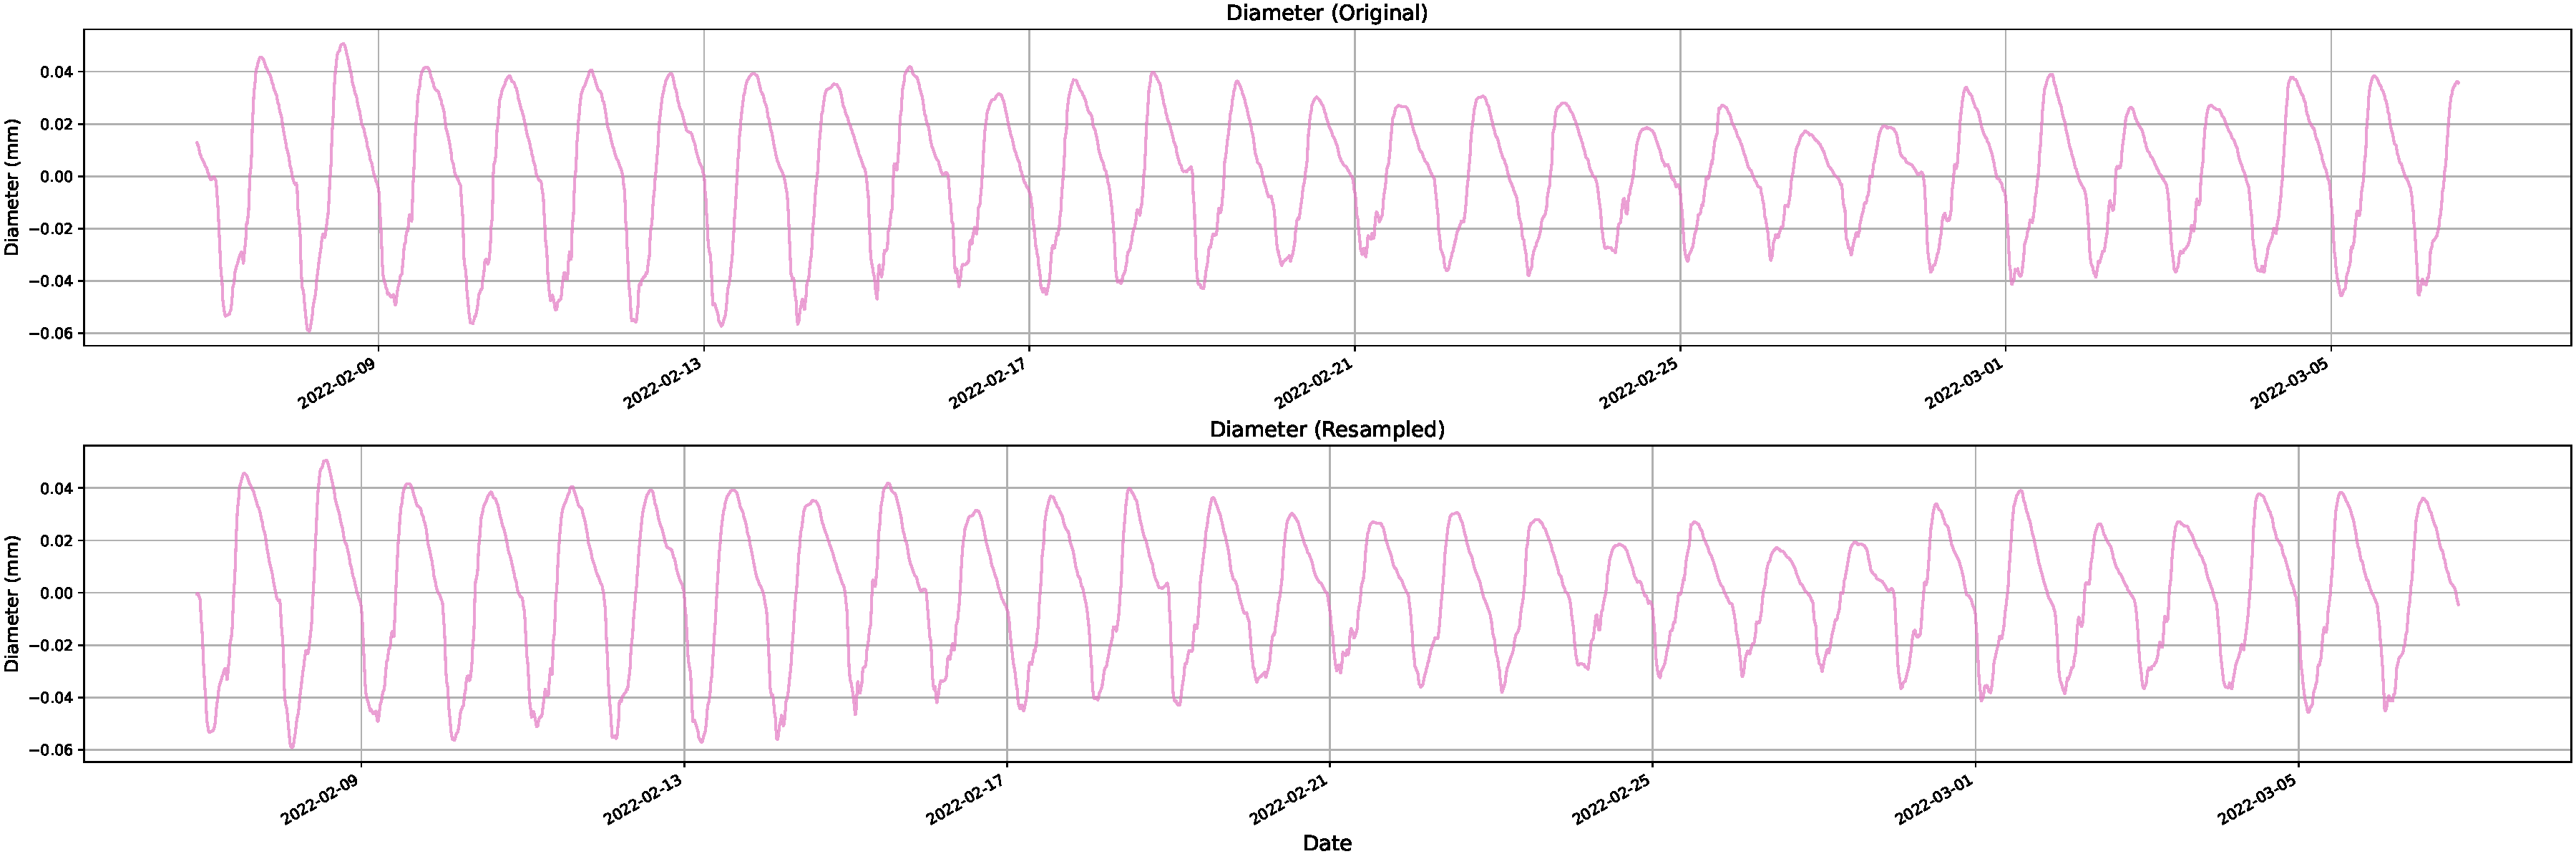
\includegraphics[width=15 cm]{5_ChapterDesign/figuras/5_Irregular/comparison_Diameter.pdf}
    \caption{Comparison of the original Diameter irregular time series and the resampled Diameter uniform time series}
    \label{comparison_Diameter}
\end{figure}

\section{Error Metrics}

This section focuses on using error measures, such as MSE and \( R^2 \), to evaluate and compare the results obtained in our study. These metrics provide a quantitative assessment of the model's accuracy and its ability to explain the variability in the observed data.

The Mean Squared Error (MSE) is a metric that quantifies the difference between the values predicted by our model and the actual observed values. It calculates the average of the squared errors and offers a measure of prediction accuracy and quality. In this context, it is transformed to a logarithmic scale to facilitate easier comparison, expressed in decibels. A more negative MSE indicates a better model. The MSE is defined as follows:

\begin{equation}
    \text{MSE} = \frac{1}{n} \sum_{i=1}^{n} \left( \text{y}_{\text{pred}_i} - \text{y}_{\text{real}_i} \right)^2
\end{equation}
    
where \( n \) represents the number of observations, \( \text{y}_{\text{pred}_i} \) is the model's predicted value for observation \( i \), and \( \text{y}_{\text{real}_i} \) is the actual observed value for observation \( i \).

On the other hand, the coefficient of determination, \( R^2 \), provides insight into the model's ability to explain the variability in the observed data. This measure is calculated by comparing the sum of squared residuals with the total sum of squares. An \( R^2 \) value close to 1 indicates a good model fit and high explanatory power, while a value near 0 suggests that the model does not adequately explain the data. The calculation of \( R^2 \) is given by:

\begin{equation}
R^2 = 1 - \frac{\text{SSE}}{\text{SST}}
\end{equation}

where SSE (Sum of Squared Errors) is the sum of the squared errors between the model's predictions and the actual observed values, and SST (Total Sum of Squares) is the sum of the squared errors between the actual values and their mean.

Relating both errors, we have:

\begin{equation}
R^2 = 1 - \frac{\text{MSE} \cdot n}{\text{SST}}
\end{equation}

Additionally, training time and the number of parameters are critical aspects in the development of neural networks. Training time impacts the model's efficiency and practical viability, affecting processing capacity, scalability, and hyperparameter optimization.

Finally, the number of parameters indicates the model's capacity to learn complex patterns but can influence overfitting, storage efficiency, and inference time. Balancing training time and the number of parameters is crucial for achieving efficient and high-performance models according to the application’s requirements and constraints.

\section{Hyperparameter Tuning}

To design an experiment for identifying a suitable time series forecasting model and analyzing various hyperparameters, we have chosen the technique known as sequential hyperparameter tuning or manual hyperparameter tuning. In this approach, we adjust one hyperparameter at a time, selecting the best model at each step before proceeding to the next hyperparameter.

This method is intuitive and offers finer control over the tuning process, which can be particularly beneficial if you have a good intuition about the relative importance of each hyperparameter. It allows for a deeper understanding of how each hyperparameter impacts the model's performance. While sequential tuning can be slower and less efficient than automated methods like grid search or random search, it simplifies the exploration of the hyperparameter space by focusing on one parameter at a time.

Sequential hyperparameter tuning is a systematic process that iteratively optimizes the parameters of a machine learning model. By keeping other parameters constant and adjusting one at a time, it helps to identify the optimal value for each hyperparameter, providing clear insights into their influence on the model's performance. This clarity is particularly valuable in applications like time series forecasting, where understanding the impact of each hyperparameter is crucial.

In this study, we conducted an experimental design involving 30 different models, changing a series of hyperparameters one by one and selecting the best at each step. Given that the study focuses on the Vanilla Transformer, Informer, and Autoformer, a total of 90 experiments were performed.

The first step in designing our experimental diagram is to choose the hyperparameters we will change and test in each part of the diagram. The selected hyperparameters are:

\begin{itemize}
    \item \textbf{Prediction Length and Context Length}
    \item \textbf{Lags Sequence}
    \item \textbf{Dropout}
    \item \textbf{Encoder Layers, Decoder Layers, and Dimensionality of the Transformer Layers}
    \item \textbf{Batch Size and Number of Epochs}
\end{itemize}

Below, the selected hyperparameters are described, along with how their values can affect the model's performance.


\subsection{Prediction Length and Context Length}

\textbf{Prediction Length:} This refers to the forecast horizon of the model, indicating how many steps into the future the model will attempt to predict. Choosing an appropriate prediction length is crucial since a horizon that is too long can lead to inaccurate predictions, while one that is too short may fail to capture important trends. Generally, this value is dictated by the dataset and the nature of the problem.

\vspace{10pt}

\noindent\textbf{Context Length:} This determines the number of past time steps the model uses to make future predictions. By default, it is equal to the prediction length but can be adjusted according to the complexity of the time series. A longer context can provide more historical information, improving prediction accuracy but also increasing computational complexity.

Figure~\ref{D1} presents the part of the experimental diagram where these values are varied, creating different configurations of these hyperparameters.

\begin{figure}[htbp]
    \centering
    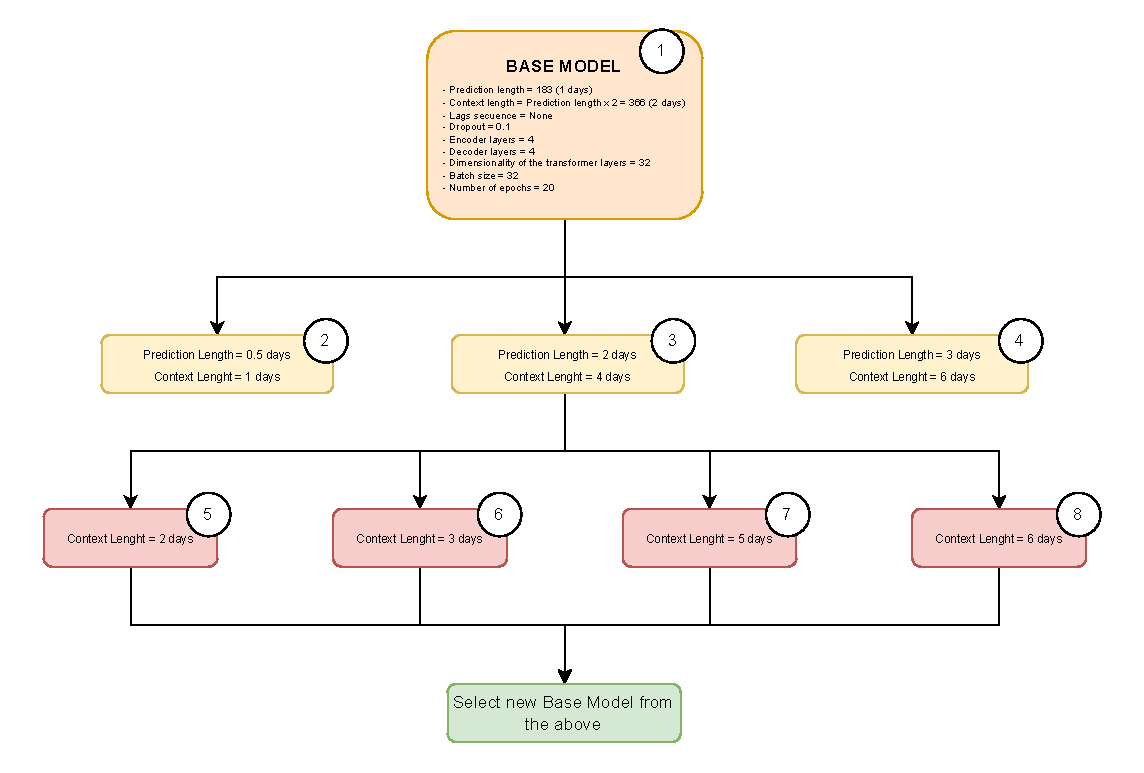
\includegraphics[width=15 cm]{5_ChapterDesign/figuras/Diagrams/D1.pdf}
    \caption{Initial Phase of the Experimental Diagram with the different Prediction Length and Context Length configurations}
    \label{D1}
\end{figure}



\subsection{Lags Sequence}

\textbf{Lags Sequence:} This defines the lags of the input time series used as covariates. This sequence is generally determined by the data's frequency. For example, if the data is daily, a common lag sequence might be [1, 2, 3, 4, 5, 6, 7], indicating that the data from the previous seven days will be used as inputs to predict the next day's value.

In our case, measurements are taken every 7 minutes and 52 seconds, so it is important to calculate the number of measurements that occur in a day. A full day has 24 hours, which equates to a total of 86,400 seconds (calculated as \(24 \, \text{hours} \times 60 \, \text{minutes per hour} \times 60 \, \text{seconds per minute}\)). Since each measurement is taken every 472 seconds (i.e., every 7 minutes and 52 seconds), we can calculate the number of daily measurements by dividing the total seconds in a day by the time interval between measurements: 

\[
\frac{86,400}{472} \approx 183
\]

This means that approximately 183 measurements are made in a day.

This specific frequency implies that to capture a complete daily cycle, we should consider a lag covering approximately 183 intervals. By adjusting the lag sequence, we can ensure that the model has enough historical information to capture complete daily patterns. Changing this sequence can affect the model's ability to capture important temporal patterns. Using appropriate lags allows the model to consider recurrent patterns in the time series, improving forecast accuracy.

Figure~\ref{D2} presents the part of the experimental diagram where these values are varied, creating different configurations of these hyperparameters.

\begin{figure}[htbp]
    \centering
    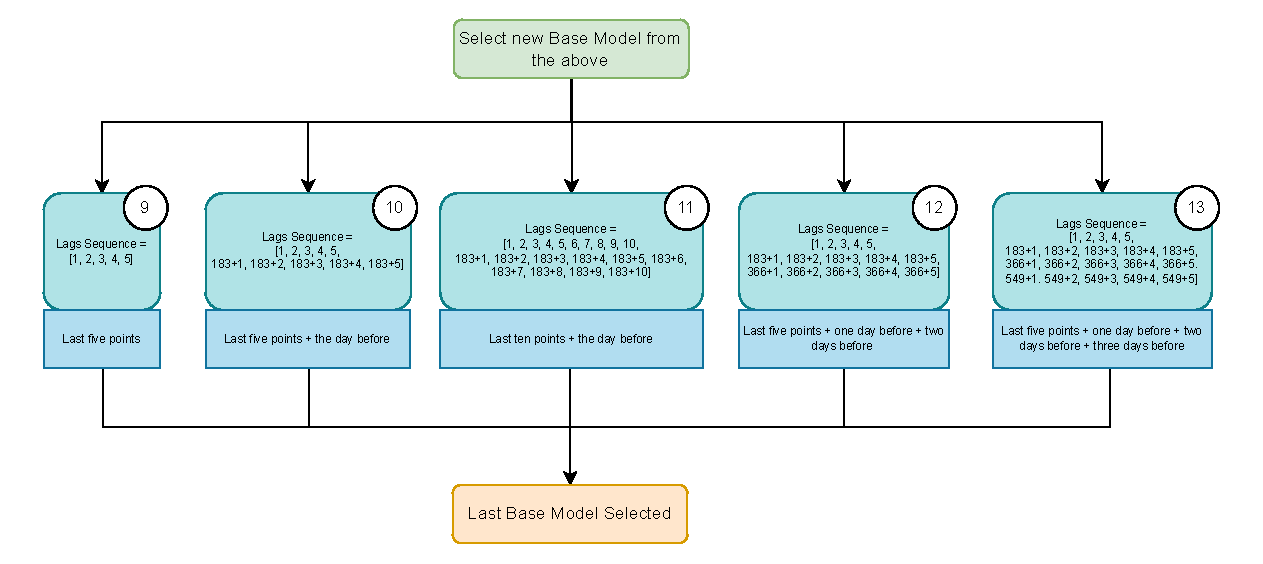
\includegraphics[width=15 cm]{5_ChapterDesign/figuras/Diagrams/D2.pdf}
    \caption{Second Phase of the Experimental Diagram with the different Lags sequence configurations}
    \label{D2}
\end{figure}

\subsection{Dropout}
\textbf{Dropout:}  This is a regularization technique used to prevent overfitting in transformers. During training, a certain percentage of nodes in the attention layers or feed-forward layers are randomly “dropped out,” meaning they are deactivated in each iteration. This means that in each training step, a different subset of nodes is turned off, which helps prevent the model from relying too heavily on any specific feature and promotes model robustness. The dropout value is specified as a fraction between 0 and 1, where higher values indicate a greater percentage of nodes being deactivated. Although too high a value can lead to poor model performance due to excessive loss of information, an appropriate value helps improve the model’s ability to generalize to unseen data.

Figure~\ref{D3} presents the part of the experimental diagram where these values are varied, creating different configurations of these hyperparameters.

\begin{figure}[htbp]
    \centering
    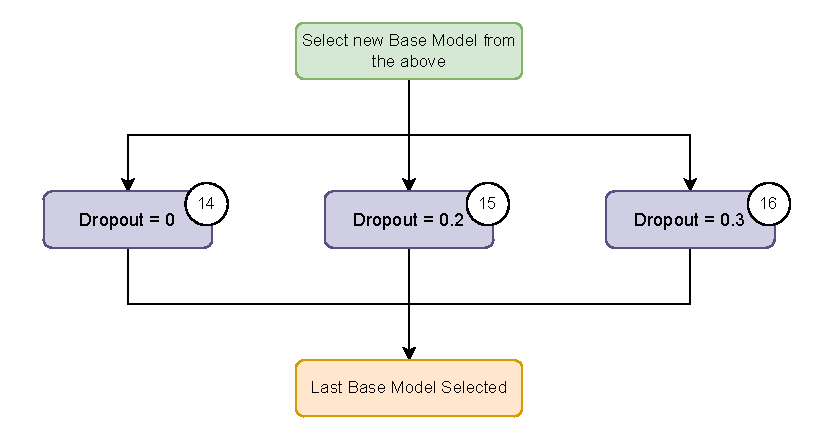
\includegraphics[width=13 cm]{5_ChapterDesign/figuras/Diagrams/D3.pdf}
    \caption{Third Phase of the Experimental Diagram with the different Dropout configurations}
    \label{D3}
\end{figure}

\subsection{Encoder Layers, Decoder Layers, and Dimensionality of the Transformer Layers}

\textbf{Dimensionality of the Transformer Layers (\(d_{model}\)):} This parameter defines the dimension of the Transformer's layers. A larger dimensionality allows the model to capture more complex representations of the time series but also increases computational cost and the risk of overfitting.

\vspace{10pt}

\noindent\textbf{Encoder Layers:} This specifies the number of layers in the Transformer's encoder. More layers can enhance the model's capacity to learn complex patterns, but they can also lead to overfitting if insufficient training data is available.

\vspace{10pt}

\noindent\textbf{Decoder Layers:} Similar to the encoder layers, this parameter defines the number of layers in the decoder. The number of decoder layers affects the model's ability to process and generate output predictions. A balance between encoding and decoding layers is essential for optimal performance.

Figure~\ref{D4} presents the part of the experimental diagram where these values are varied, creating different configurations of these hyperparameters.

\begin{figure}[htbp]
    \centering
    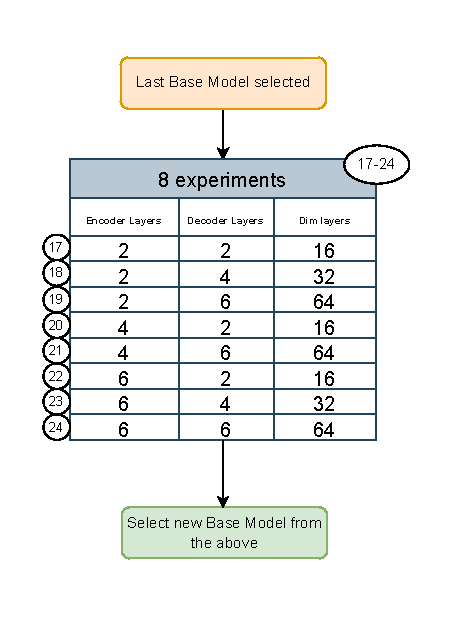
\includegraphics[width=8 cm]{5_ChapterDesign/figuras/Diagrams/D4.pdf}
    \caption{Fourth Phase of the Experimental Diagram with the different Encoder Layers, Decoder Layers, and Dimensionality of the Transformer Layers configurations}
    \label{D4}
\end{figure}


\subsection{Batch Size and Number of Epochs}

\textbf{Batch Size:} This indicates the number of samples used to update the model in each iteration. A small batch size can lead to faster convergence but with more noise, while a large batch can stabilize the training process but require more memory. The choice of batch size can influence the model's ability to generalize to new data and the total training time.

\vspace{10pt}

\noindent\textbf{Number of Epochs:} This is the number of times the model will iterate over the entire training dataset. An insufficient number of epochs may result in an underfitted model, while too many can cause overfitting. Selecting the appropriate number of epochs is essential to ensure that the model learns meaningful patterns without memorizing the noise in the training data.

Figure~\ref{D5} presents the part of the experimental diagram where these values are varied, creating different configurations of these hyperparameters.

\begin{figure}[htbp]
    \centering
    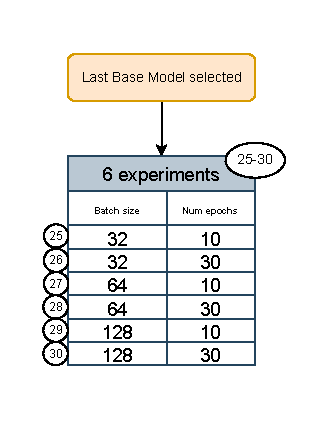
\includegraphics[width=7 cm]{5_ChapterDesign/figuras/Diagrams/D5.pdf}
    \caption{Last Phase of the Experimental Diagram with the different Batch Size and Number of Epochs configurations}
    \label{D5}
\end{figure}